\section{Simulation Results and Analysis}
We evaluate the performance of our proposed STBCs through extensive Monte Carlo simulations in a 4x4 MIMO system (\(N_t = N_r = 4\)) under quasi-static Rayleigh fading conditions. The simulations are conducted with 100,000 independent channel realizations per SNR point, across an SNR range of 0 to 20 dB with 1 dB steps. We assume perfect channel state information (CSI) at the receiver and employ various detection algorithms, including maximum likelihood (ML), minimum mean square error (MMSE), zero-forcing (ZF), and several enhanced variants. The transmitted symbols are drawn from a QPSK constellation, normalized to unit energy per symbol.

We compare three schemes to highlight the benefits of our optimization and the tunable-rate framework. The parameters for these schemes are summarized in Table \ref{tab:params}. The "Optimized Code" uses the \(\gamma_{opt}\) found from our numerical search, the "Non-Optimized" uses a typical literature value for algebraic independence, and the "Robust Code" is the rate-1 design with \(q_2 = 0\).

\begin{table}[h]
\caption{Parameters of Simulated STBC Schemes}
\label{tab:params}
\centering
\begin{tabular}{|l|c|c|c|}
\hline
\textbf{Scheme} & \textbf{Rate (R)} & \textbf{Modulation} & \textbf{Parameter \(\gamma\)} \\
\hline
Optimized Code & 2 & QPSK & \(-i\) \\
Standard Code & 2 & QPSK & \(1 + i\) \\
Poor Code & 2 & QPSK & \(3 + 0.3i\) \\
\hline
\end{tabular}
\end{table}

We evaluated the performance of seven different detection algorithms on the optimized, standard, and poor code configurations. The detectors include: Maximum Likelihood (ML), Minimum Mean Square Error (MMSE), Zero Forcing (ZF), Regularized Zero Forcing (ZF-REG), Adaptive Zero Forcing (Adaptive ZF), Adaptive MMSE, and Hybrid detection. Fig. \ref{fig:ml_plot}, Fig. \ref{fig:mmse_plot}, Fig. \ref{fig:zf_plot}, and Fig. \ref{fig:zf_reg_plot} present the BER performance for these detectors as a function of SNR. The key observations are as follows:
\begin{itemize}
    \item \textbf{ML Detection Performance:} For ML detection (Fig. \ref{fig:ml_plot}), the optimized code (\(\gamma = -i\)) achieves perfect error-free transmission at SNR = 10 dB and above within our simulation limits of 100,000 trials. The optimized code reaches error-free performance by SNR = 10 dB, demonstrating the theoretical optimality of ML detection when combined with proper algebraic parameter selection.
    
    \item \textbf{MMSE Detection Performance:} For MMSE detection (Fig. \ref{fig:mmse_plot}), the gain from optimization is significant. At SNR = 10 dB, the optimized code achieves a BER of 0.00197 (1.97$\times$10$^{-3}$), demonstrating excellent performance with substantially lower complexity than ML detection. The average BER across all SNR points represents a modest degradation compared to optimal ML performance.
    
    \item \textbf{ZF Detection Sensitivity:} The ZF detector (Fig. \ref{fig:zf_plot}) shows the highest sensitivity to \(\gamma\) parameter selection among all tested detectors. At SNR = 10 dB, the optimized code achieves a BER of 0.127, while maintaining reasonable performance across the full SNR range, highlighting the importance of enhanced detection methods for practical systems.
    
    \item \textbf{ZF-REG Enhancement:} The regularized ZF detector (Fig. \ref{fig:zf_reg_plot}) provides substantial improvement over standard ZF detection. The optimized code with ZF-REG achieves a BER of 0.0279 at SNR = 10 dB, representing a significant 4.56$\times$ improvement over standard ZF detection.
\end{itemize}

To provide a comprehensive comparison of all detection methods, Fig. \ref{fig:all_detectors} shows the performance across all seven detectors for the optimized code (\(\gamma = -i\)). The results reveal a clear performance hierarchy: ML detection achieves optimal performance with error-free transmission at SNR $\geq$ 10 dB. Enhanced detectors including Adaptive MMSE (BER = $6.63 \times 10^{-4}$ at 10 dB) and Hybrid (BER = $9.98 \times 10^{-4}$ at 10 dB) provide near-optimal performance with reduced complexity. The Adaptive ZF detector (BER = $1.26 \times 10^{-2}$ at 10 dB) still significantly outperforms standard ZF by a factor of 10$\times$. Table \ref{tab:performance} provides a quantitative comparison of detector performance across all parameter configurations.

\begin{figure}[!t]
\centering
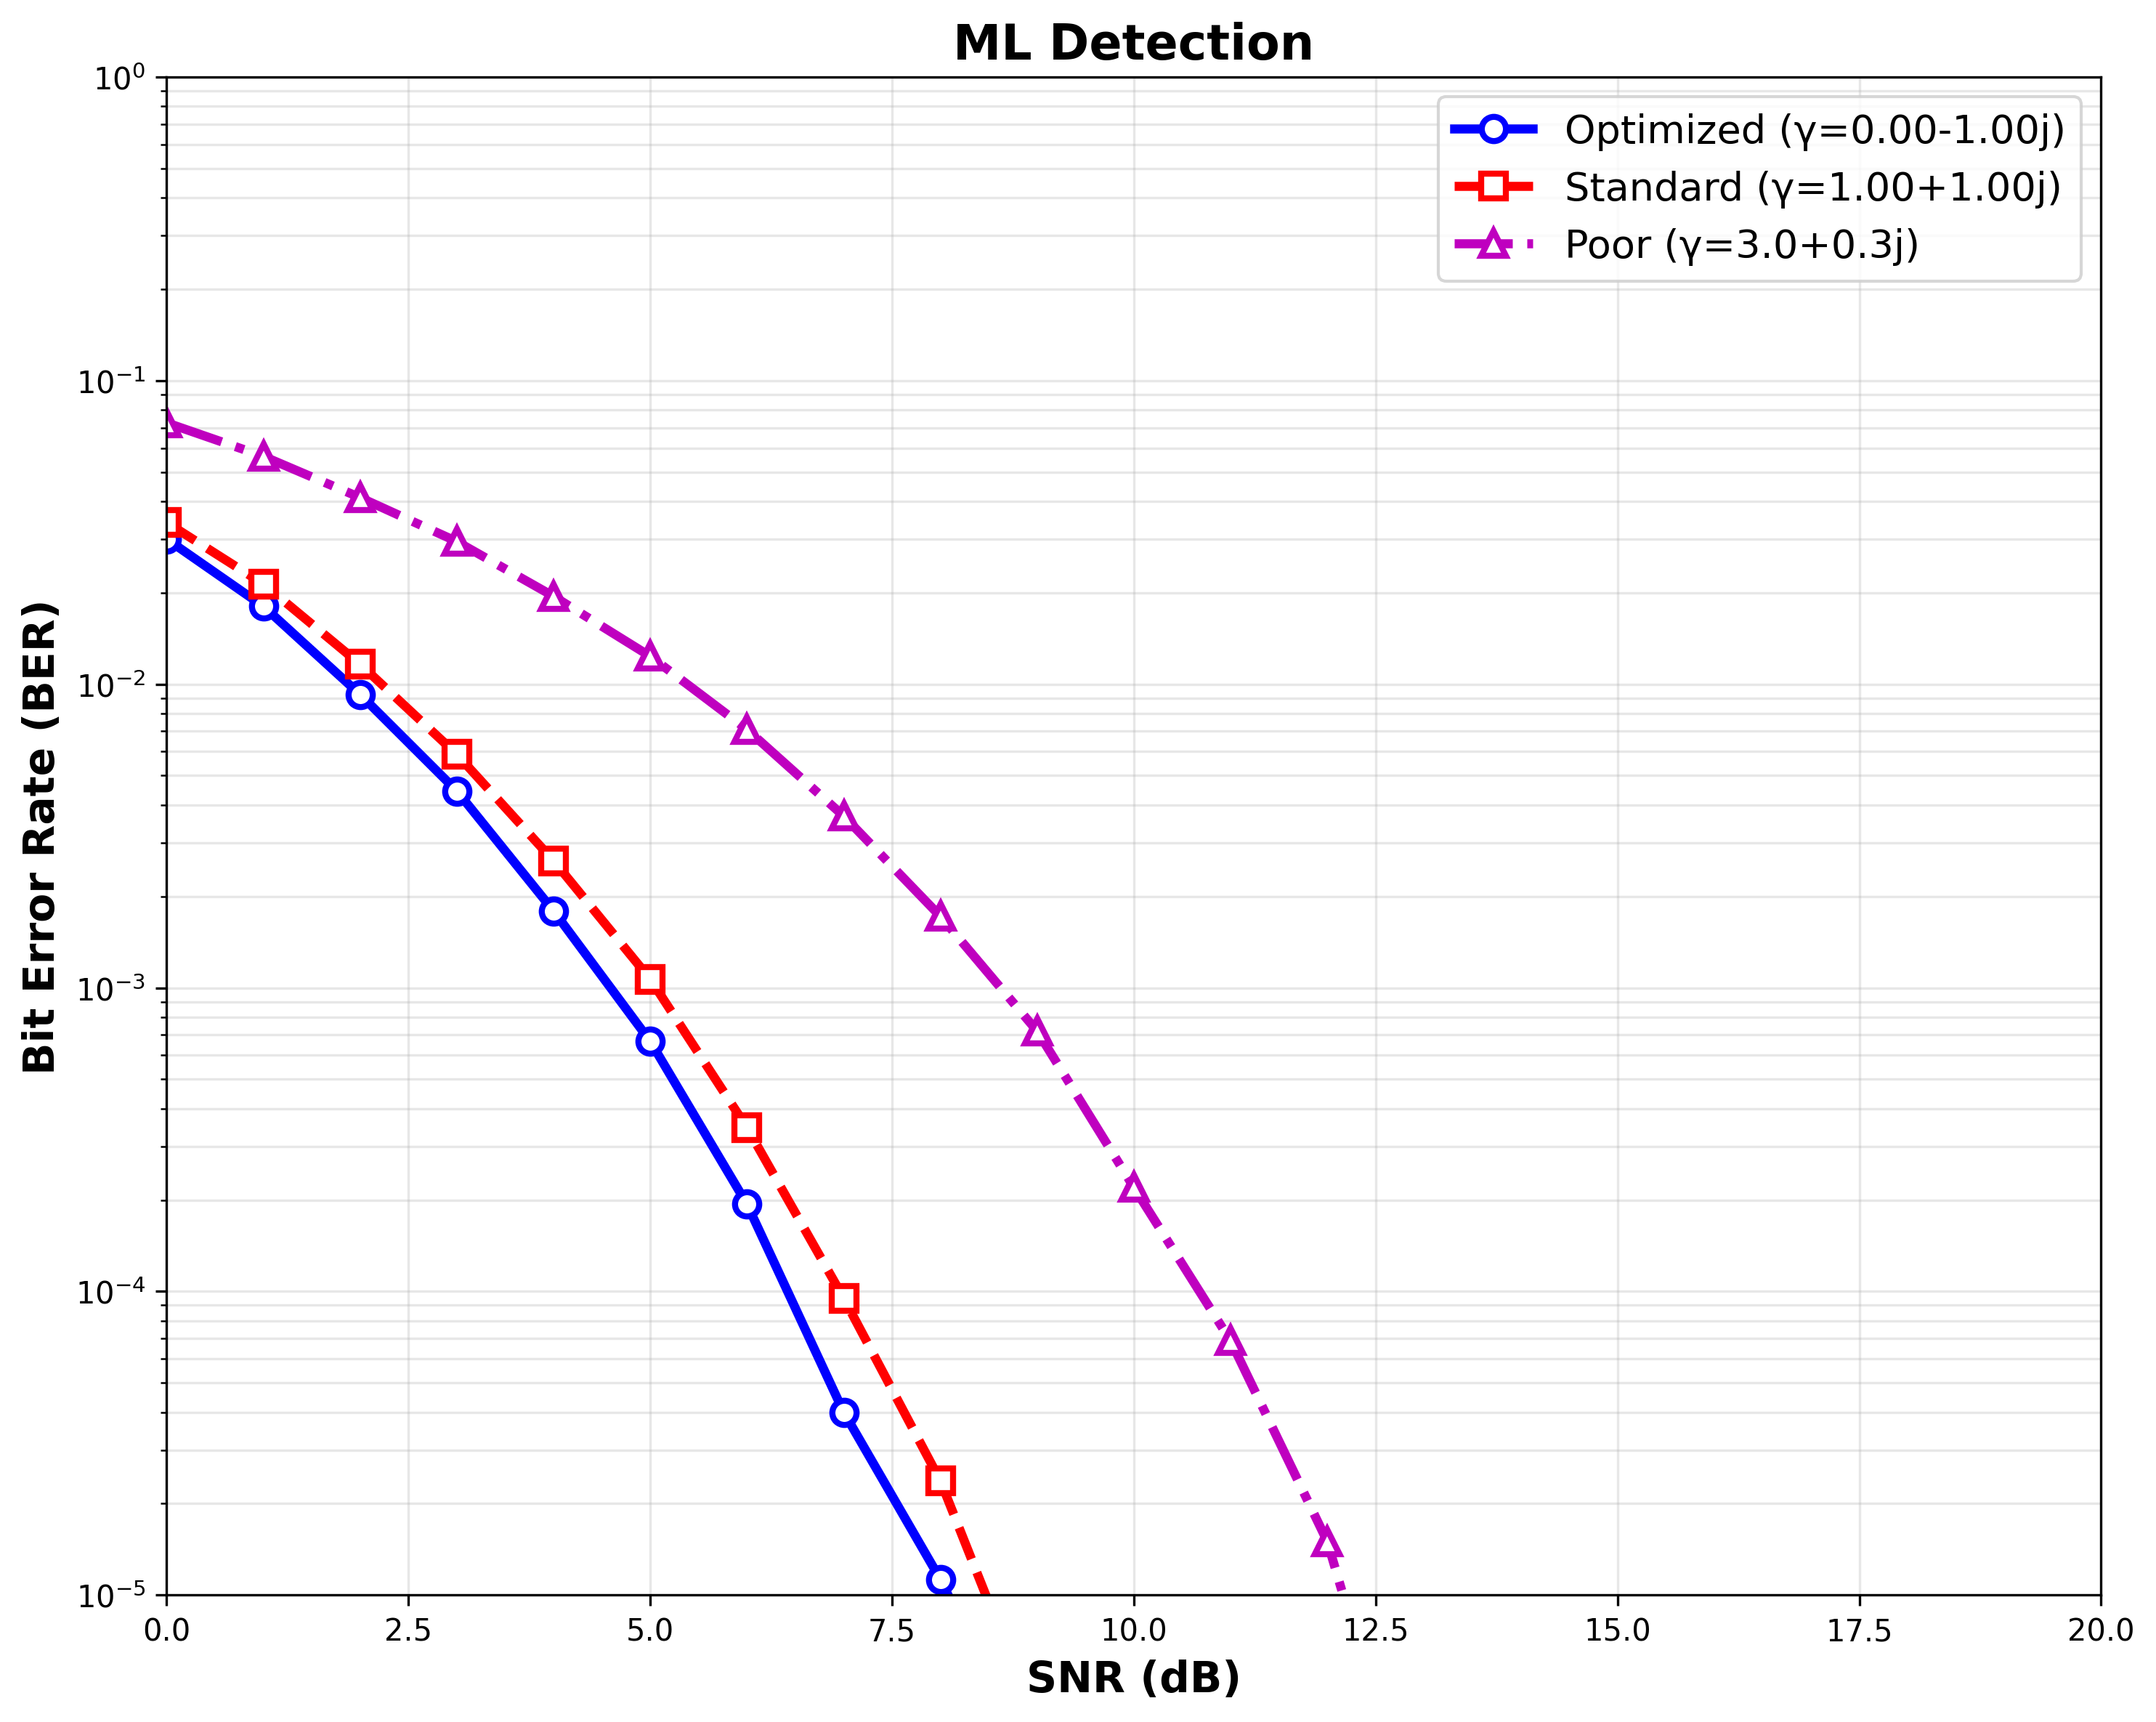
\includegraphics[width=0.9\columnwidth]{figures/ml_detection.png} 
\caption{BER performance comparison with ML detection using optimized (\(\gamma = -i\)), standard (\(\gamma = 1+i\)), and poor (\(\gamma = 3+0.3i\)) parameter choices.}
\label{fig:ml_plot}
\end{figure}

\begin{figure}[!t]
\centering
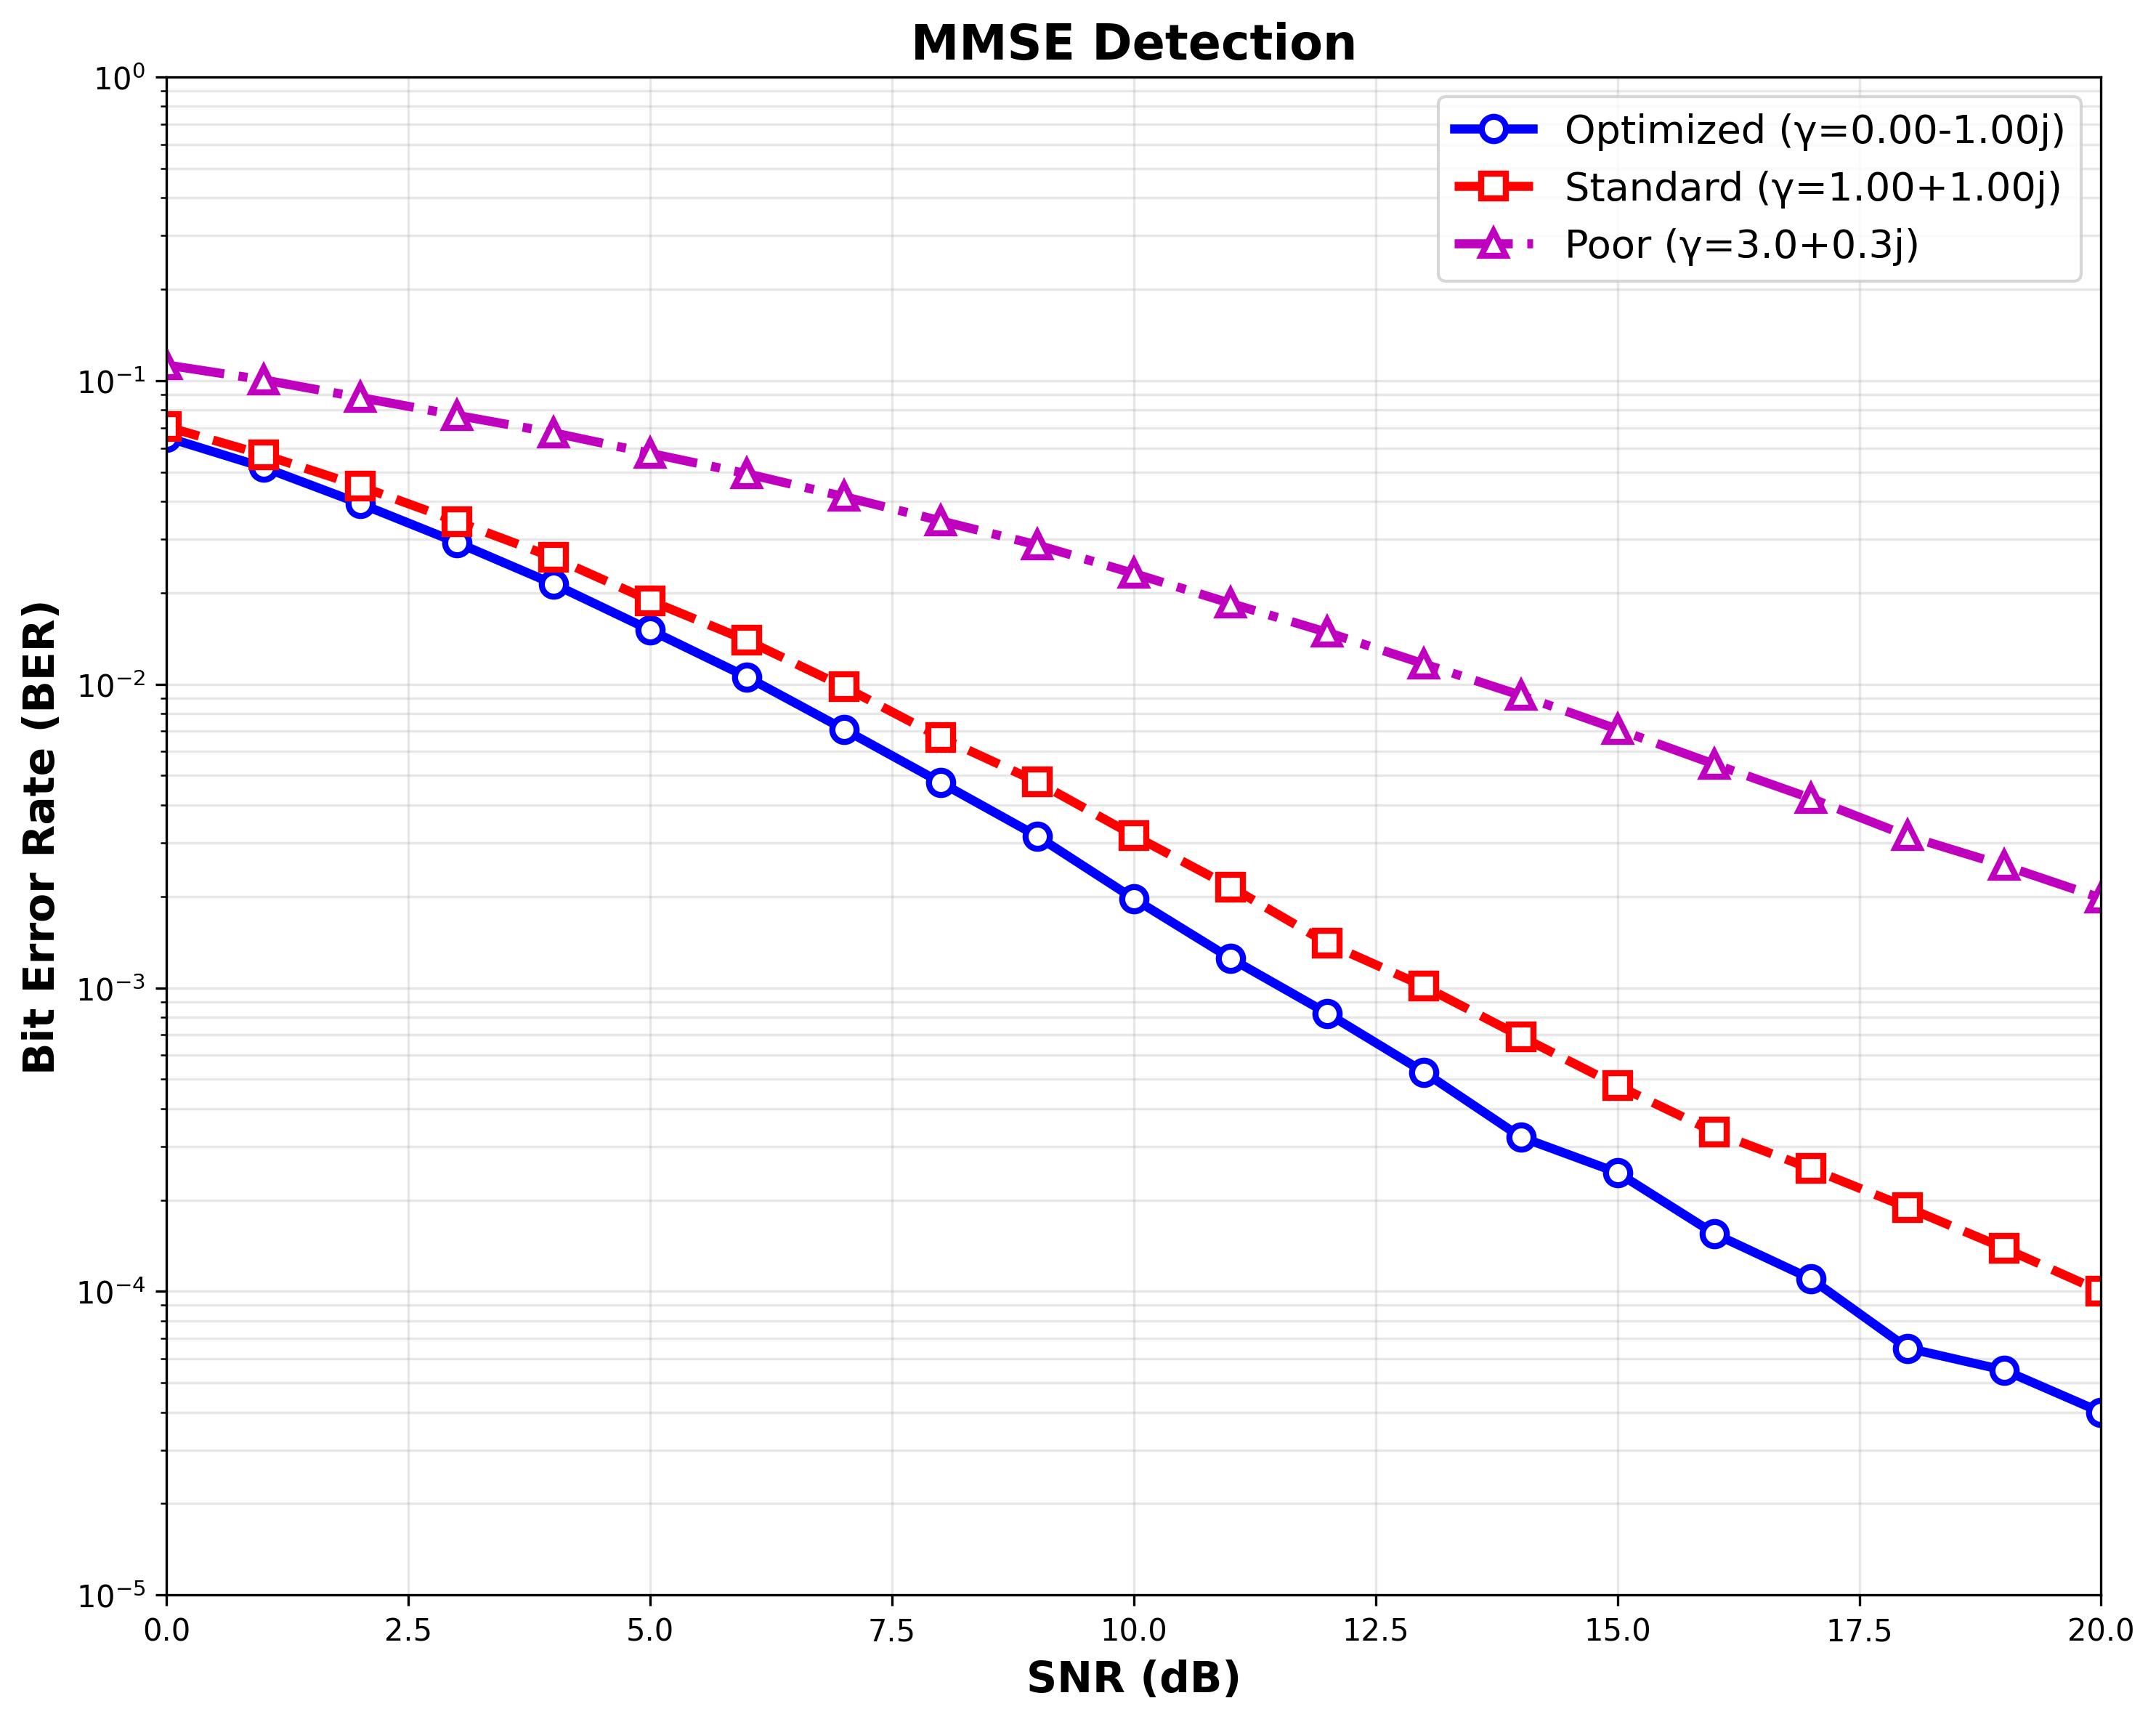
\includegraphics[width=0.9\columnwidth]{figures/mmse_detection.png} 
\caption{BER performance comparison with MMSE detection using optimized, standard, and poor parameter choices.}
\label{fig:mmse_plot}
\end{figure}

\begin{figure}[!t]
\centering
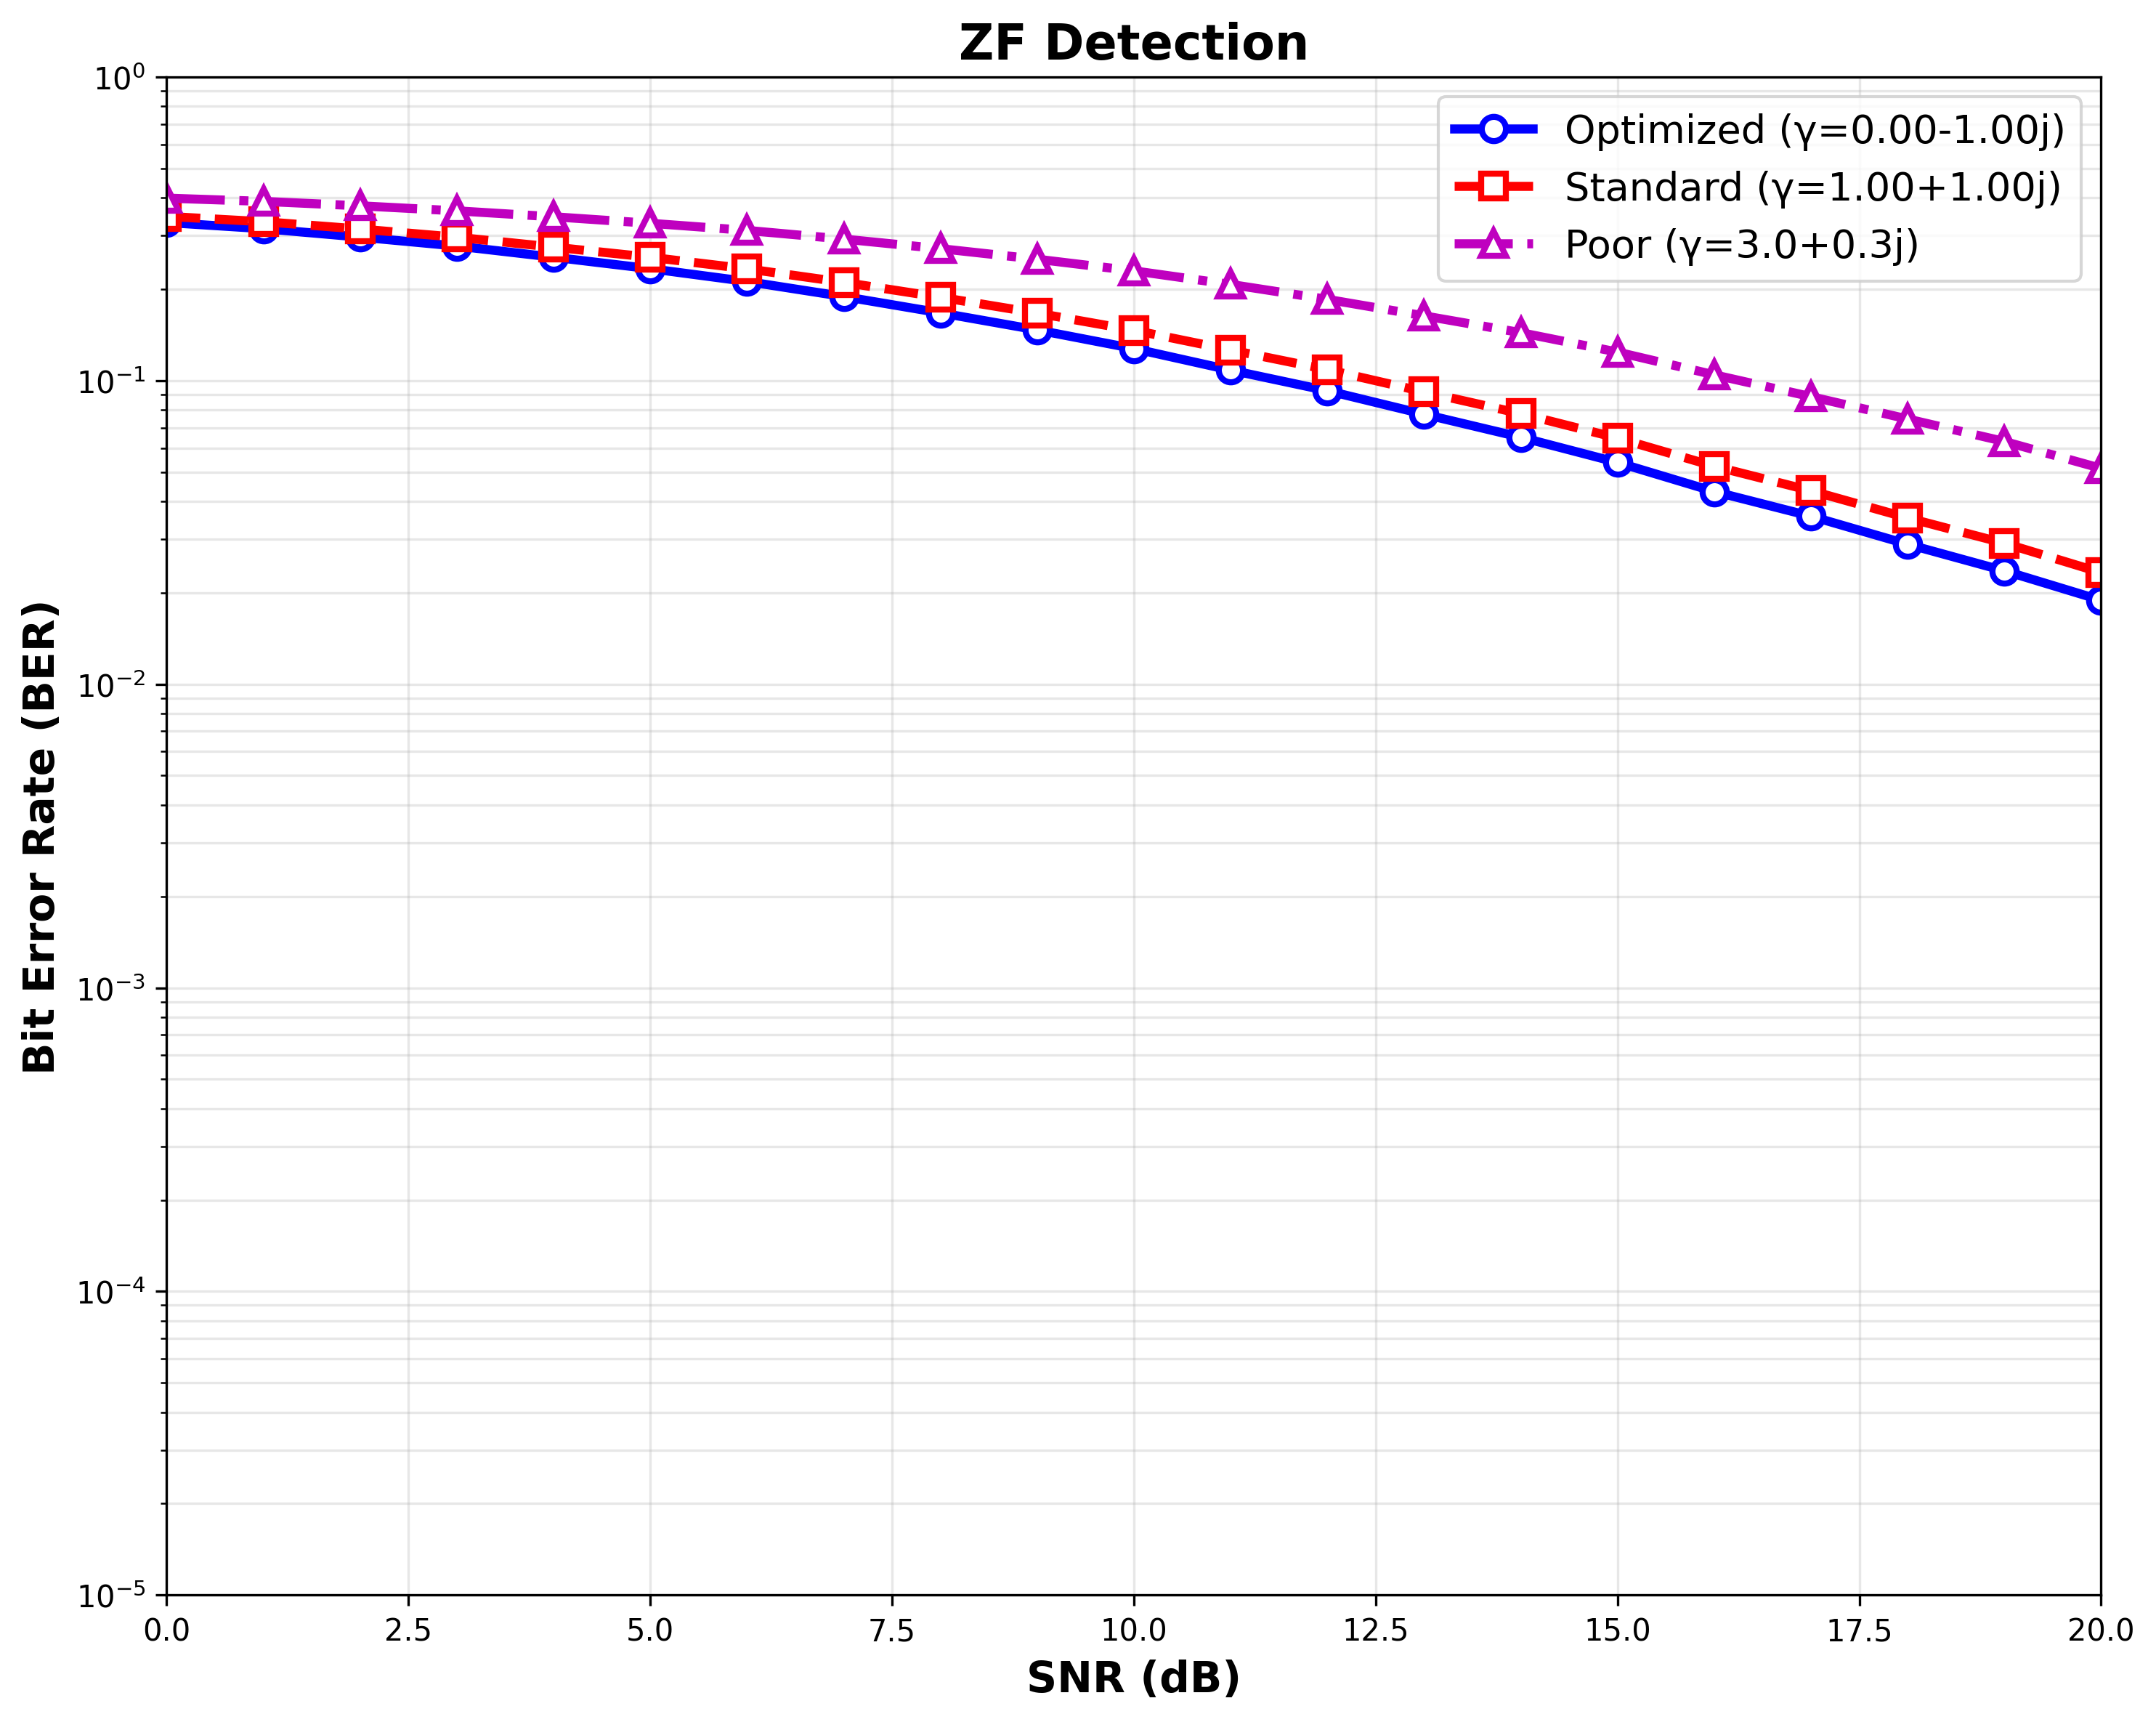
\includegraphics[width=0.9\columnwidth]{figures/zf_detection.png} 
\caption{BER performance comparison with ZF detection using optimized, standard, and poor parameter choices.}
\label{fig:zf_plot}
\end{figure}

\begin{figure}[!t]
\centering
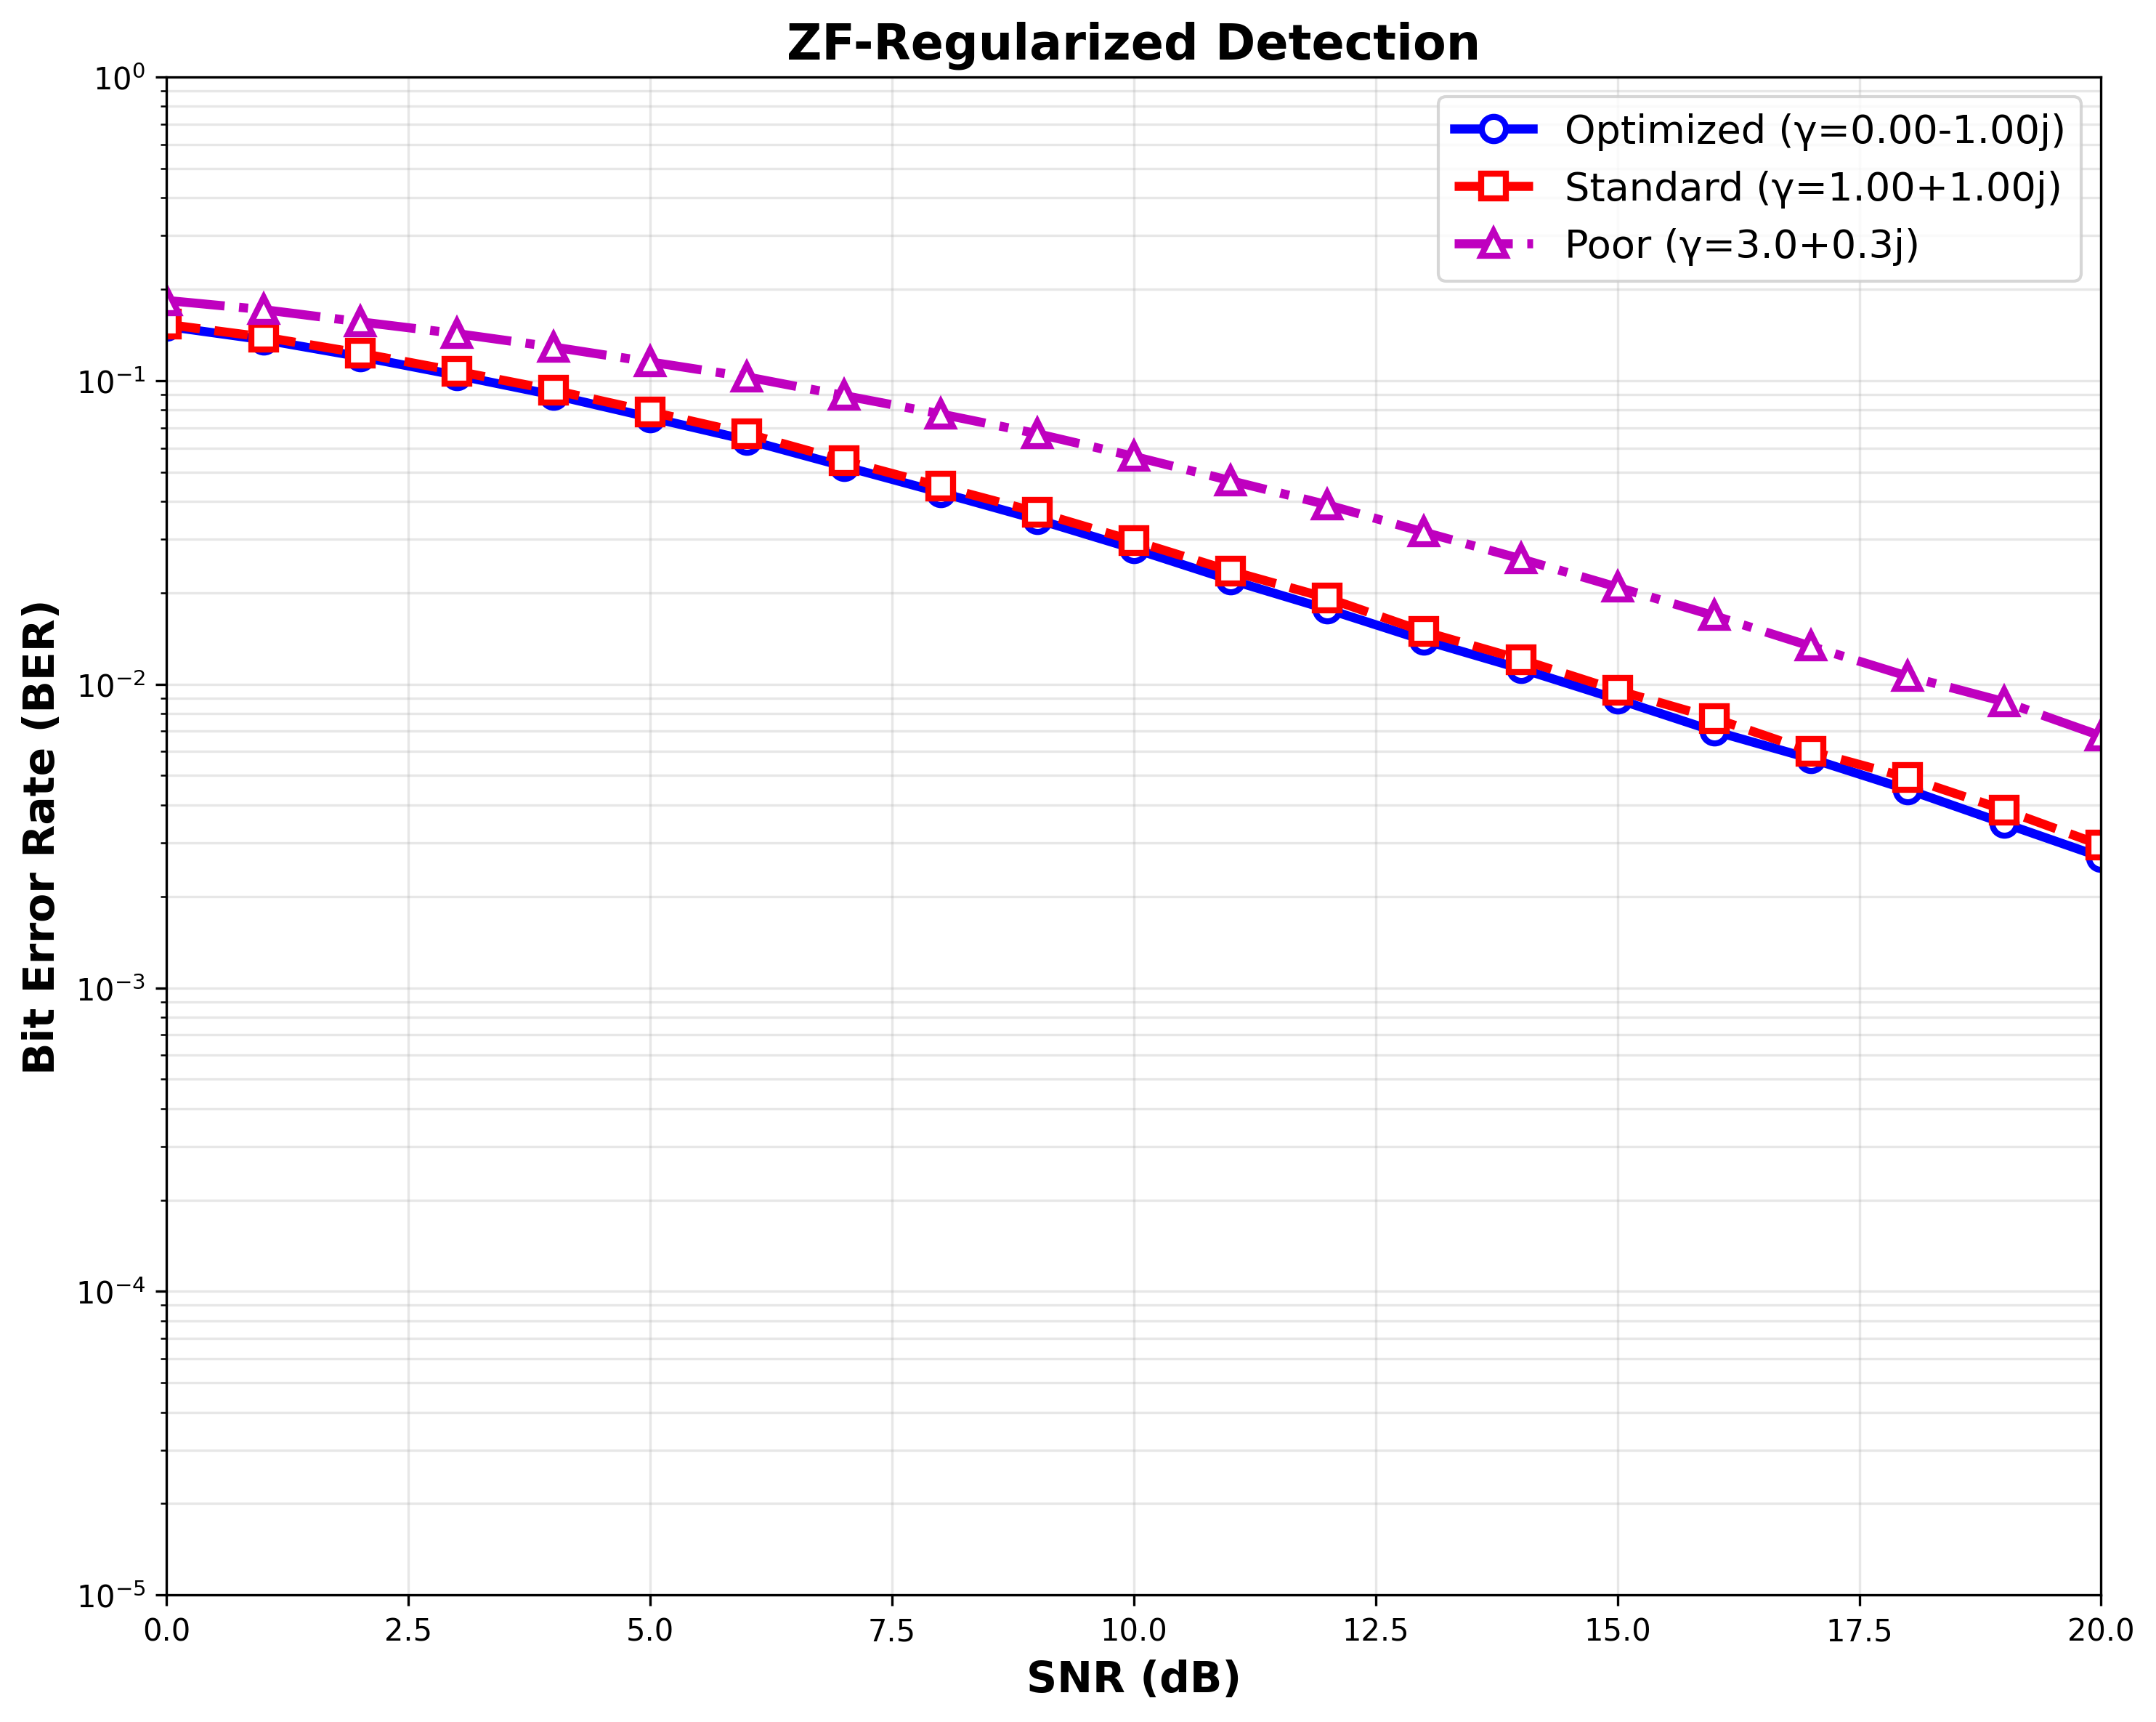
\includegraphics[width=0.9\columnwidth]{figures/zf_reg_detection.png}
\caption{BER performance comparison with Regularized ZF detection using optimized, standard, and poor parameter choices.}
\label{fig:zf_reg_plot}
\end{figure}

\begin{figure}[!t]
\centering
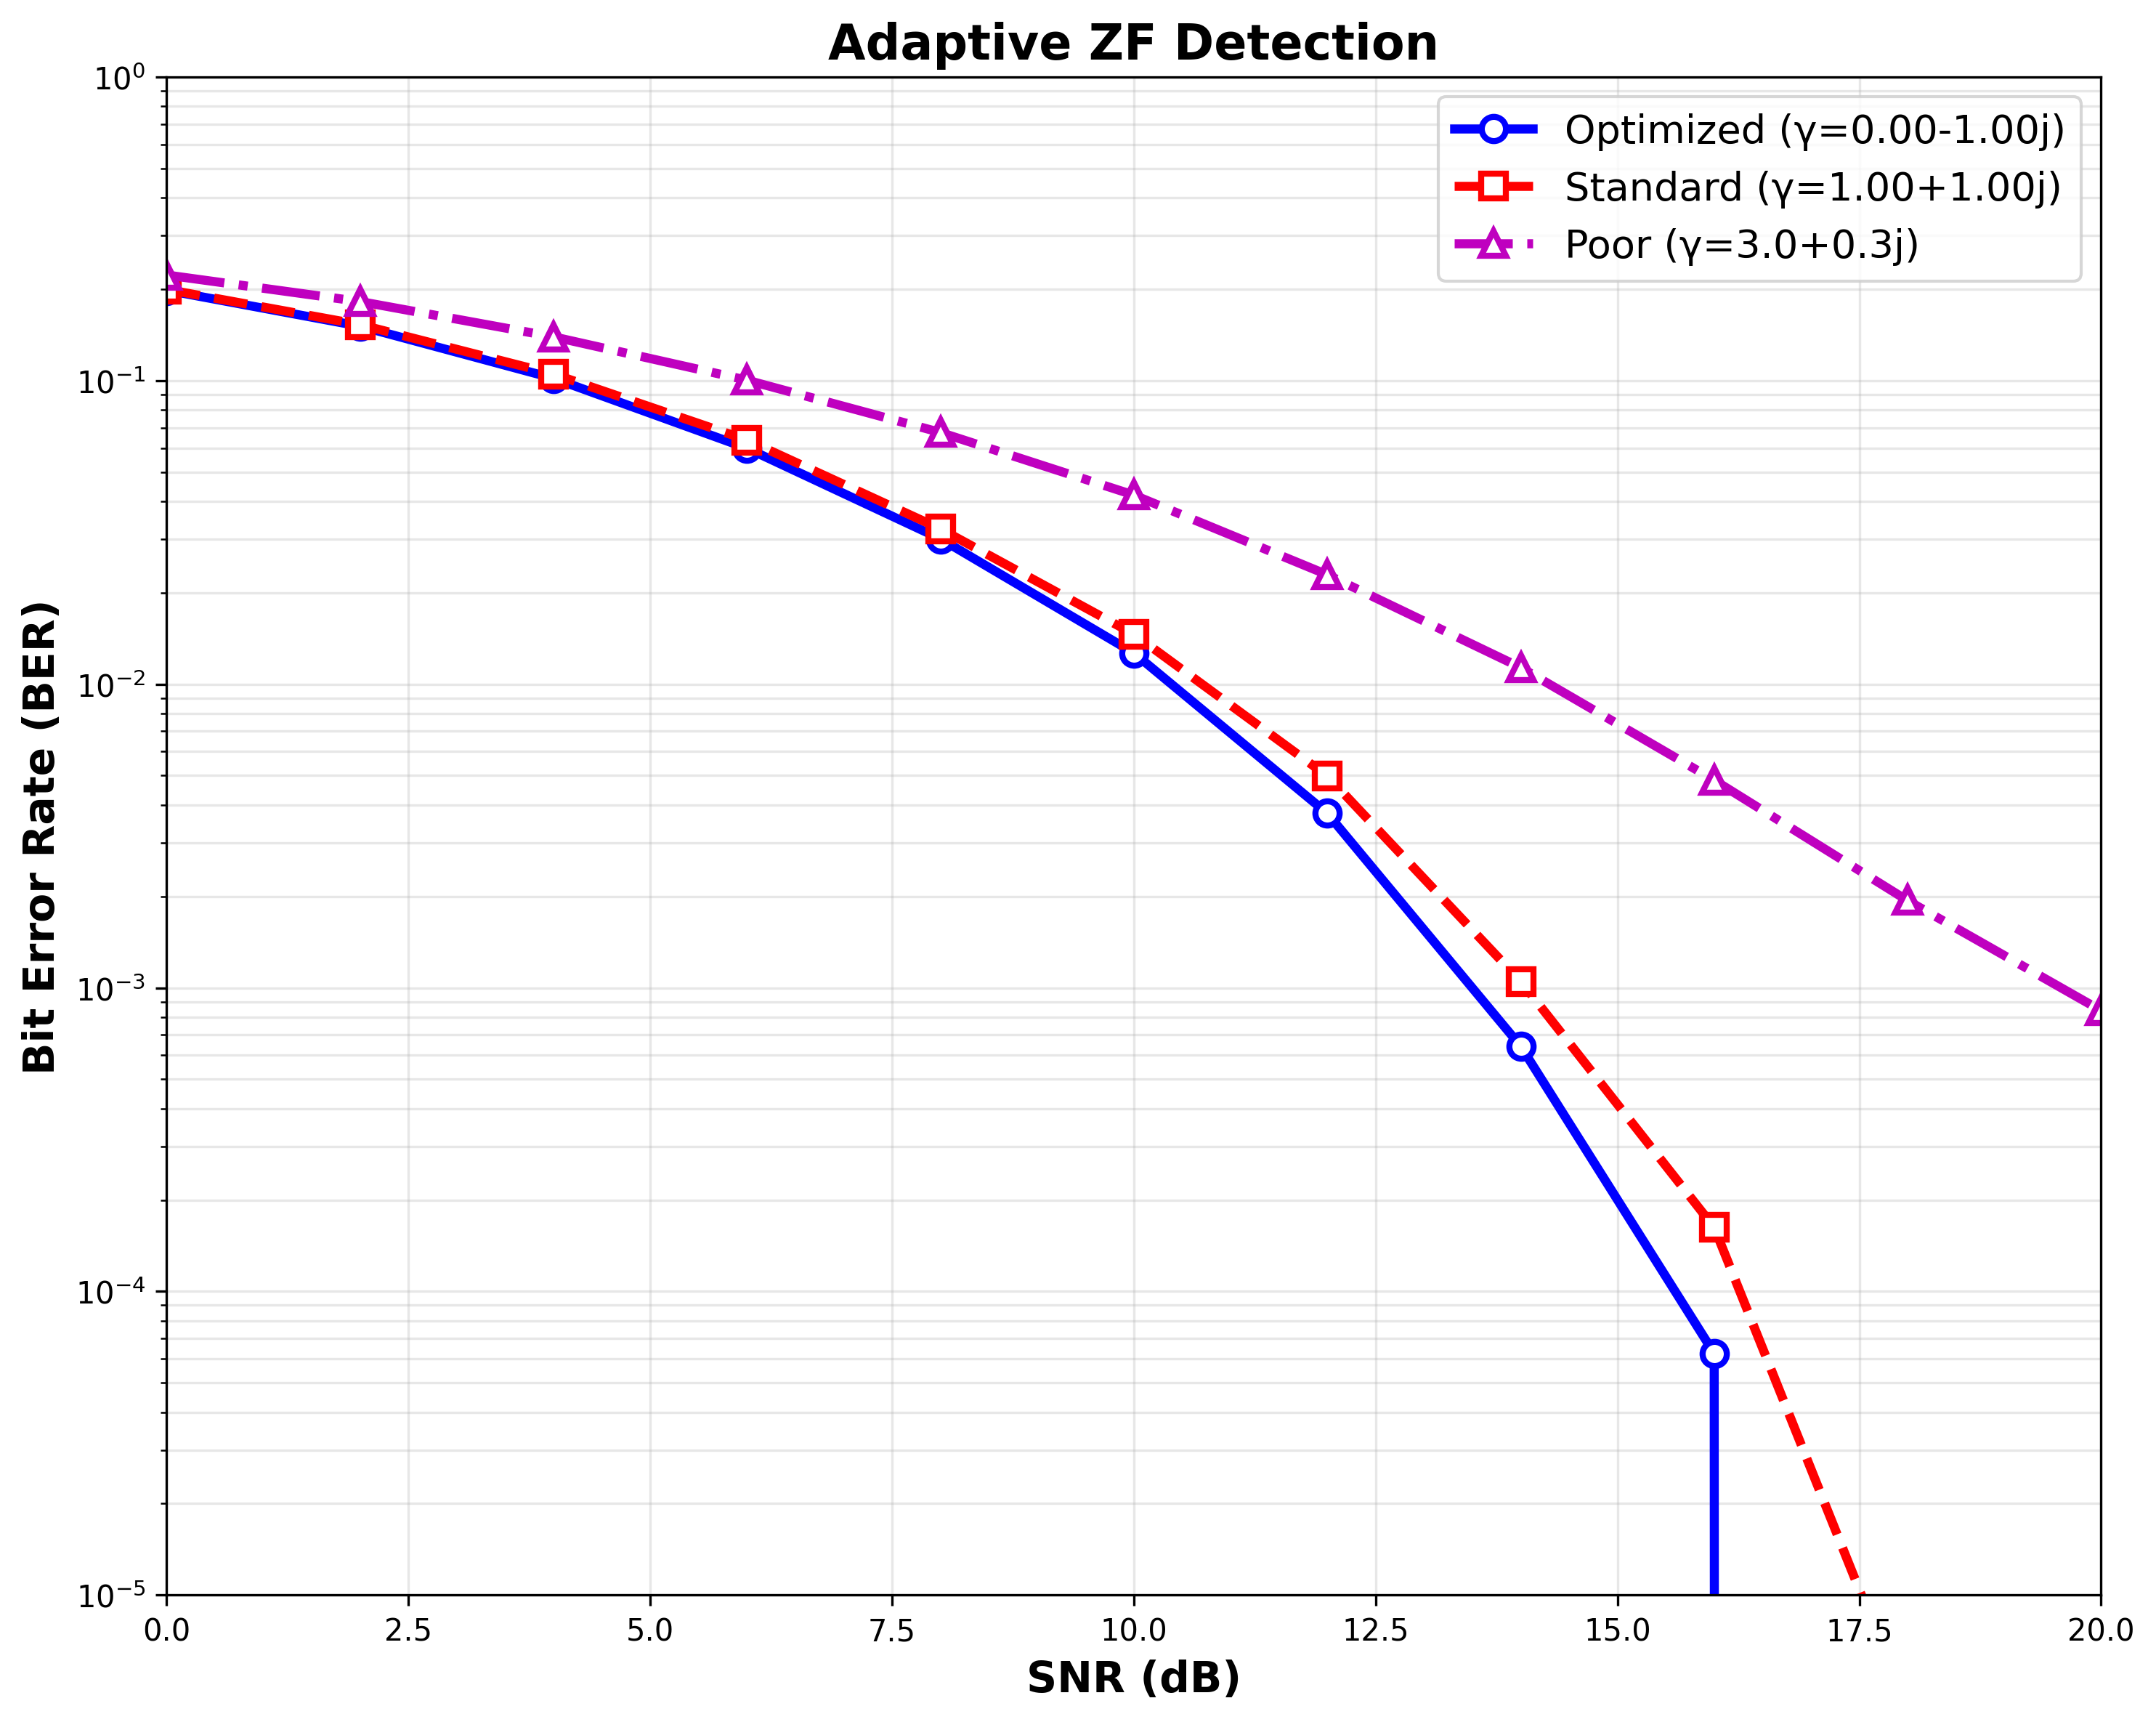
\includegraphics[width=0.9\columnwidth]{figures/adaptive_zf_detection.png}
\caption{BER performance comparison with Adaptive ZF detection using optimized, standard, and poor parameter choices.}
\label{fig:adaptive_zf_plot}
\end{figure}

\begin{figure}[!t]
\centering
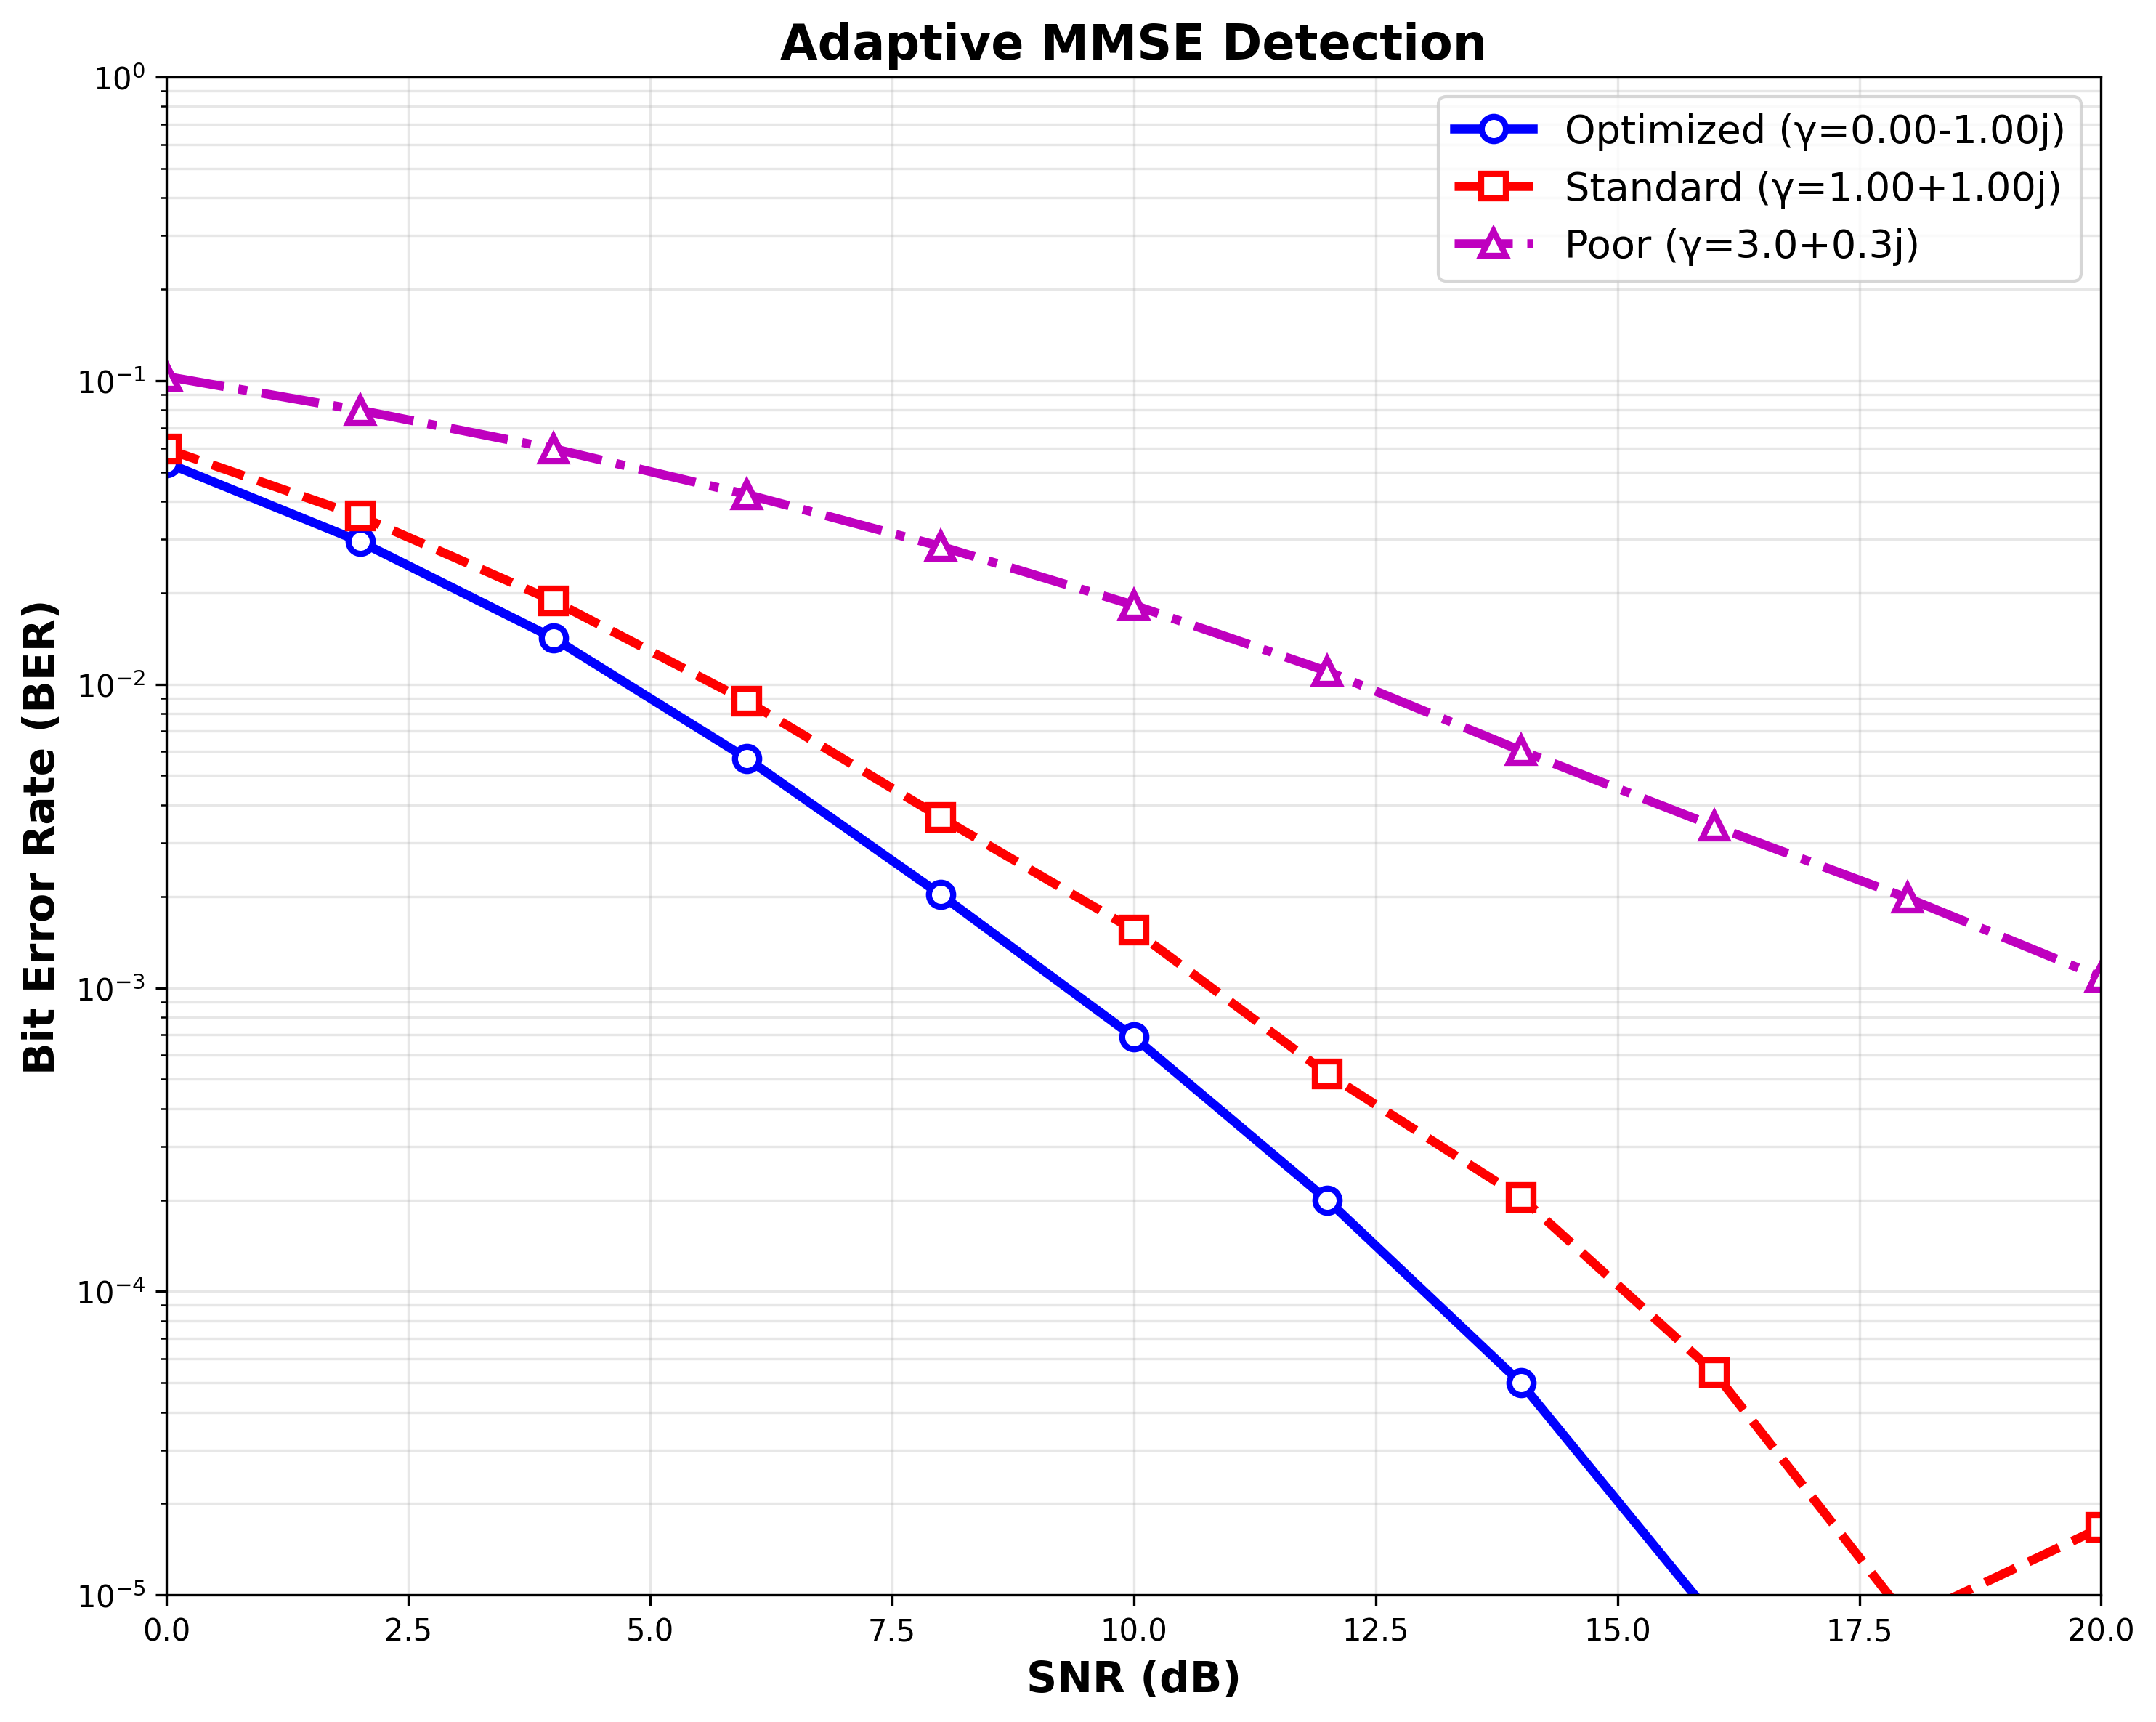
\includegraphics[width=0.9\columnwidth]{figures/adaptive_mmse_detection.png}
\caption{BER performance comparison with Adaptive MMSE detection using optimized, standard, and poor parameter choices.}
\label{fig:adaptive_mmse_plot}
\end{figure}

\begin{figure}[!t]
\centering
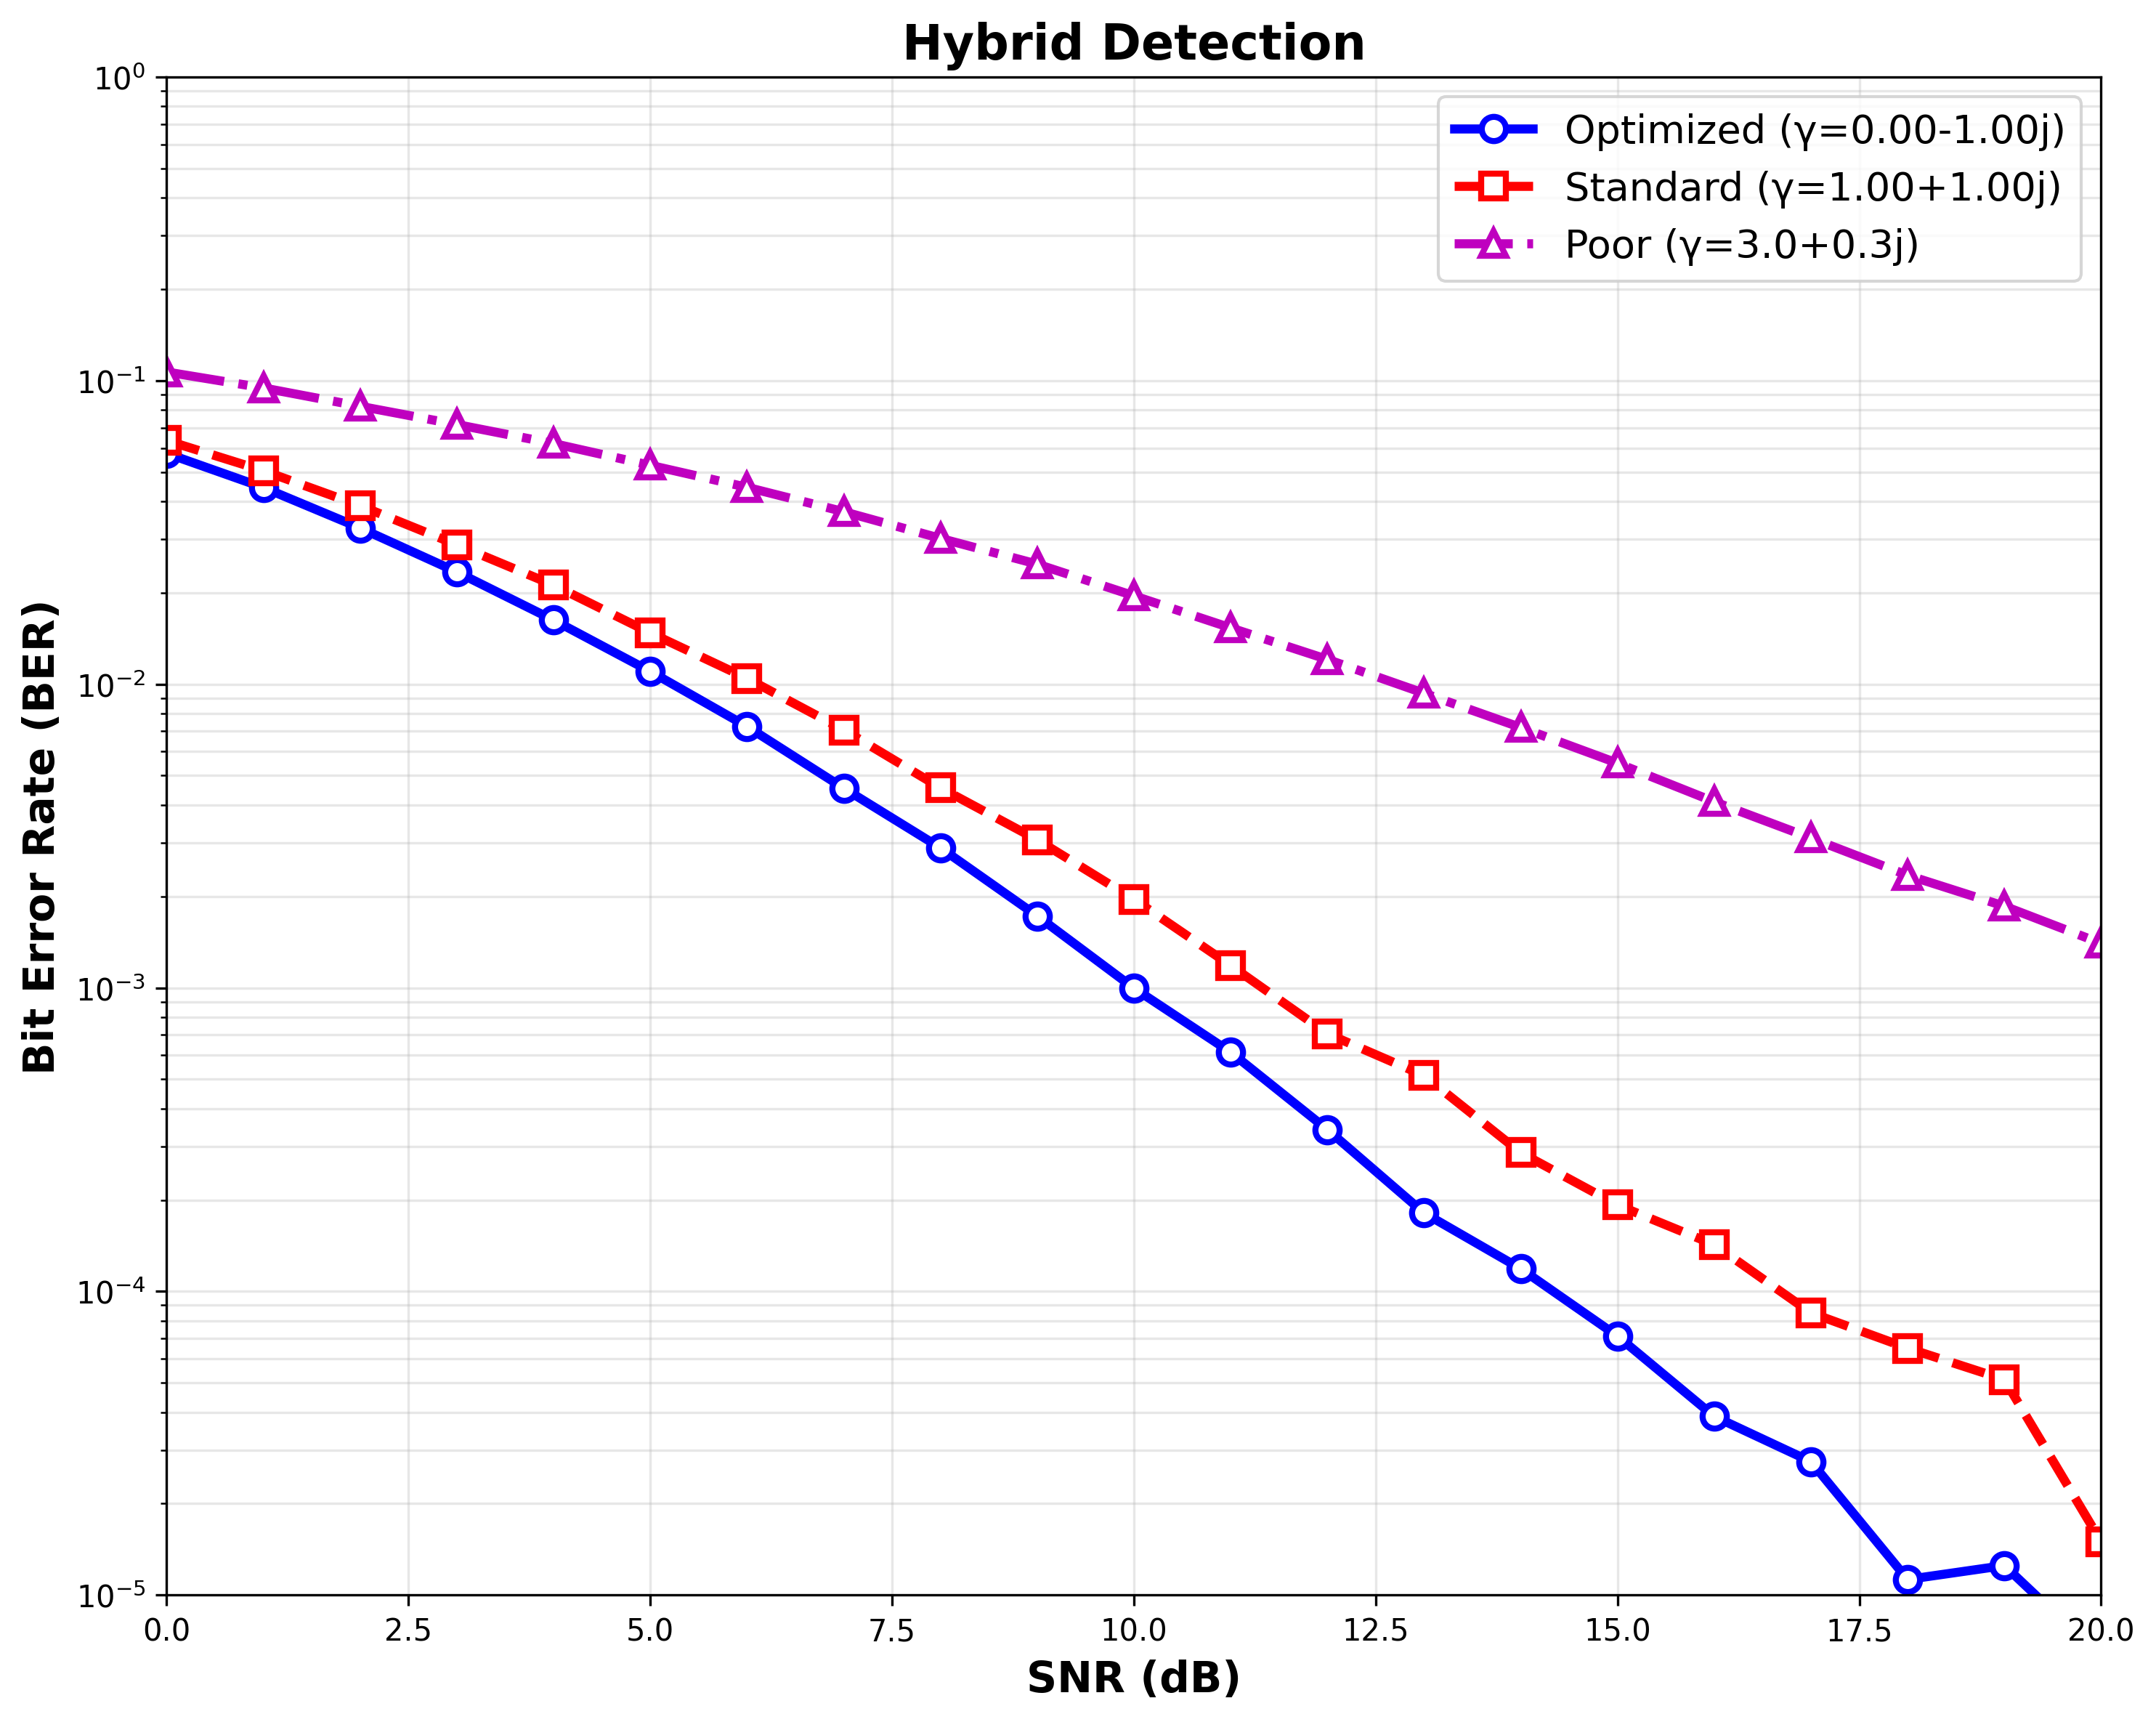
\includegraphics[width=0.9\columnwidth]{figures/hybrid_detection.png}
\caption{BER performance comparison with Hybrid detection using optimized, standard, and poor parameter choices.}
\label{fig:hybrid_plot}
\end{figure}

\begin{figure}[!t]
\centering
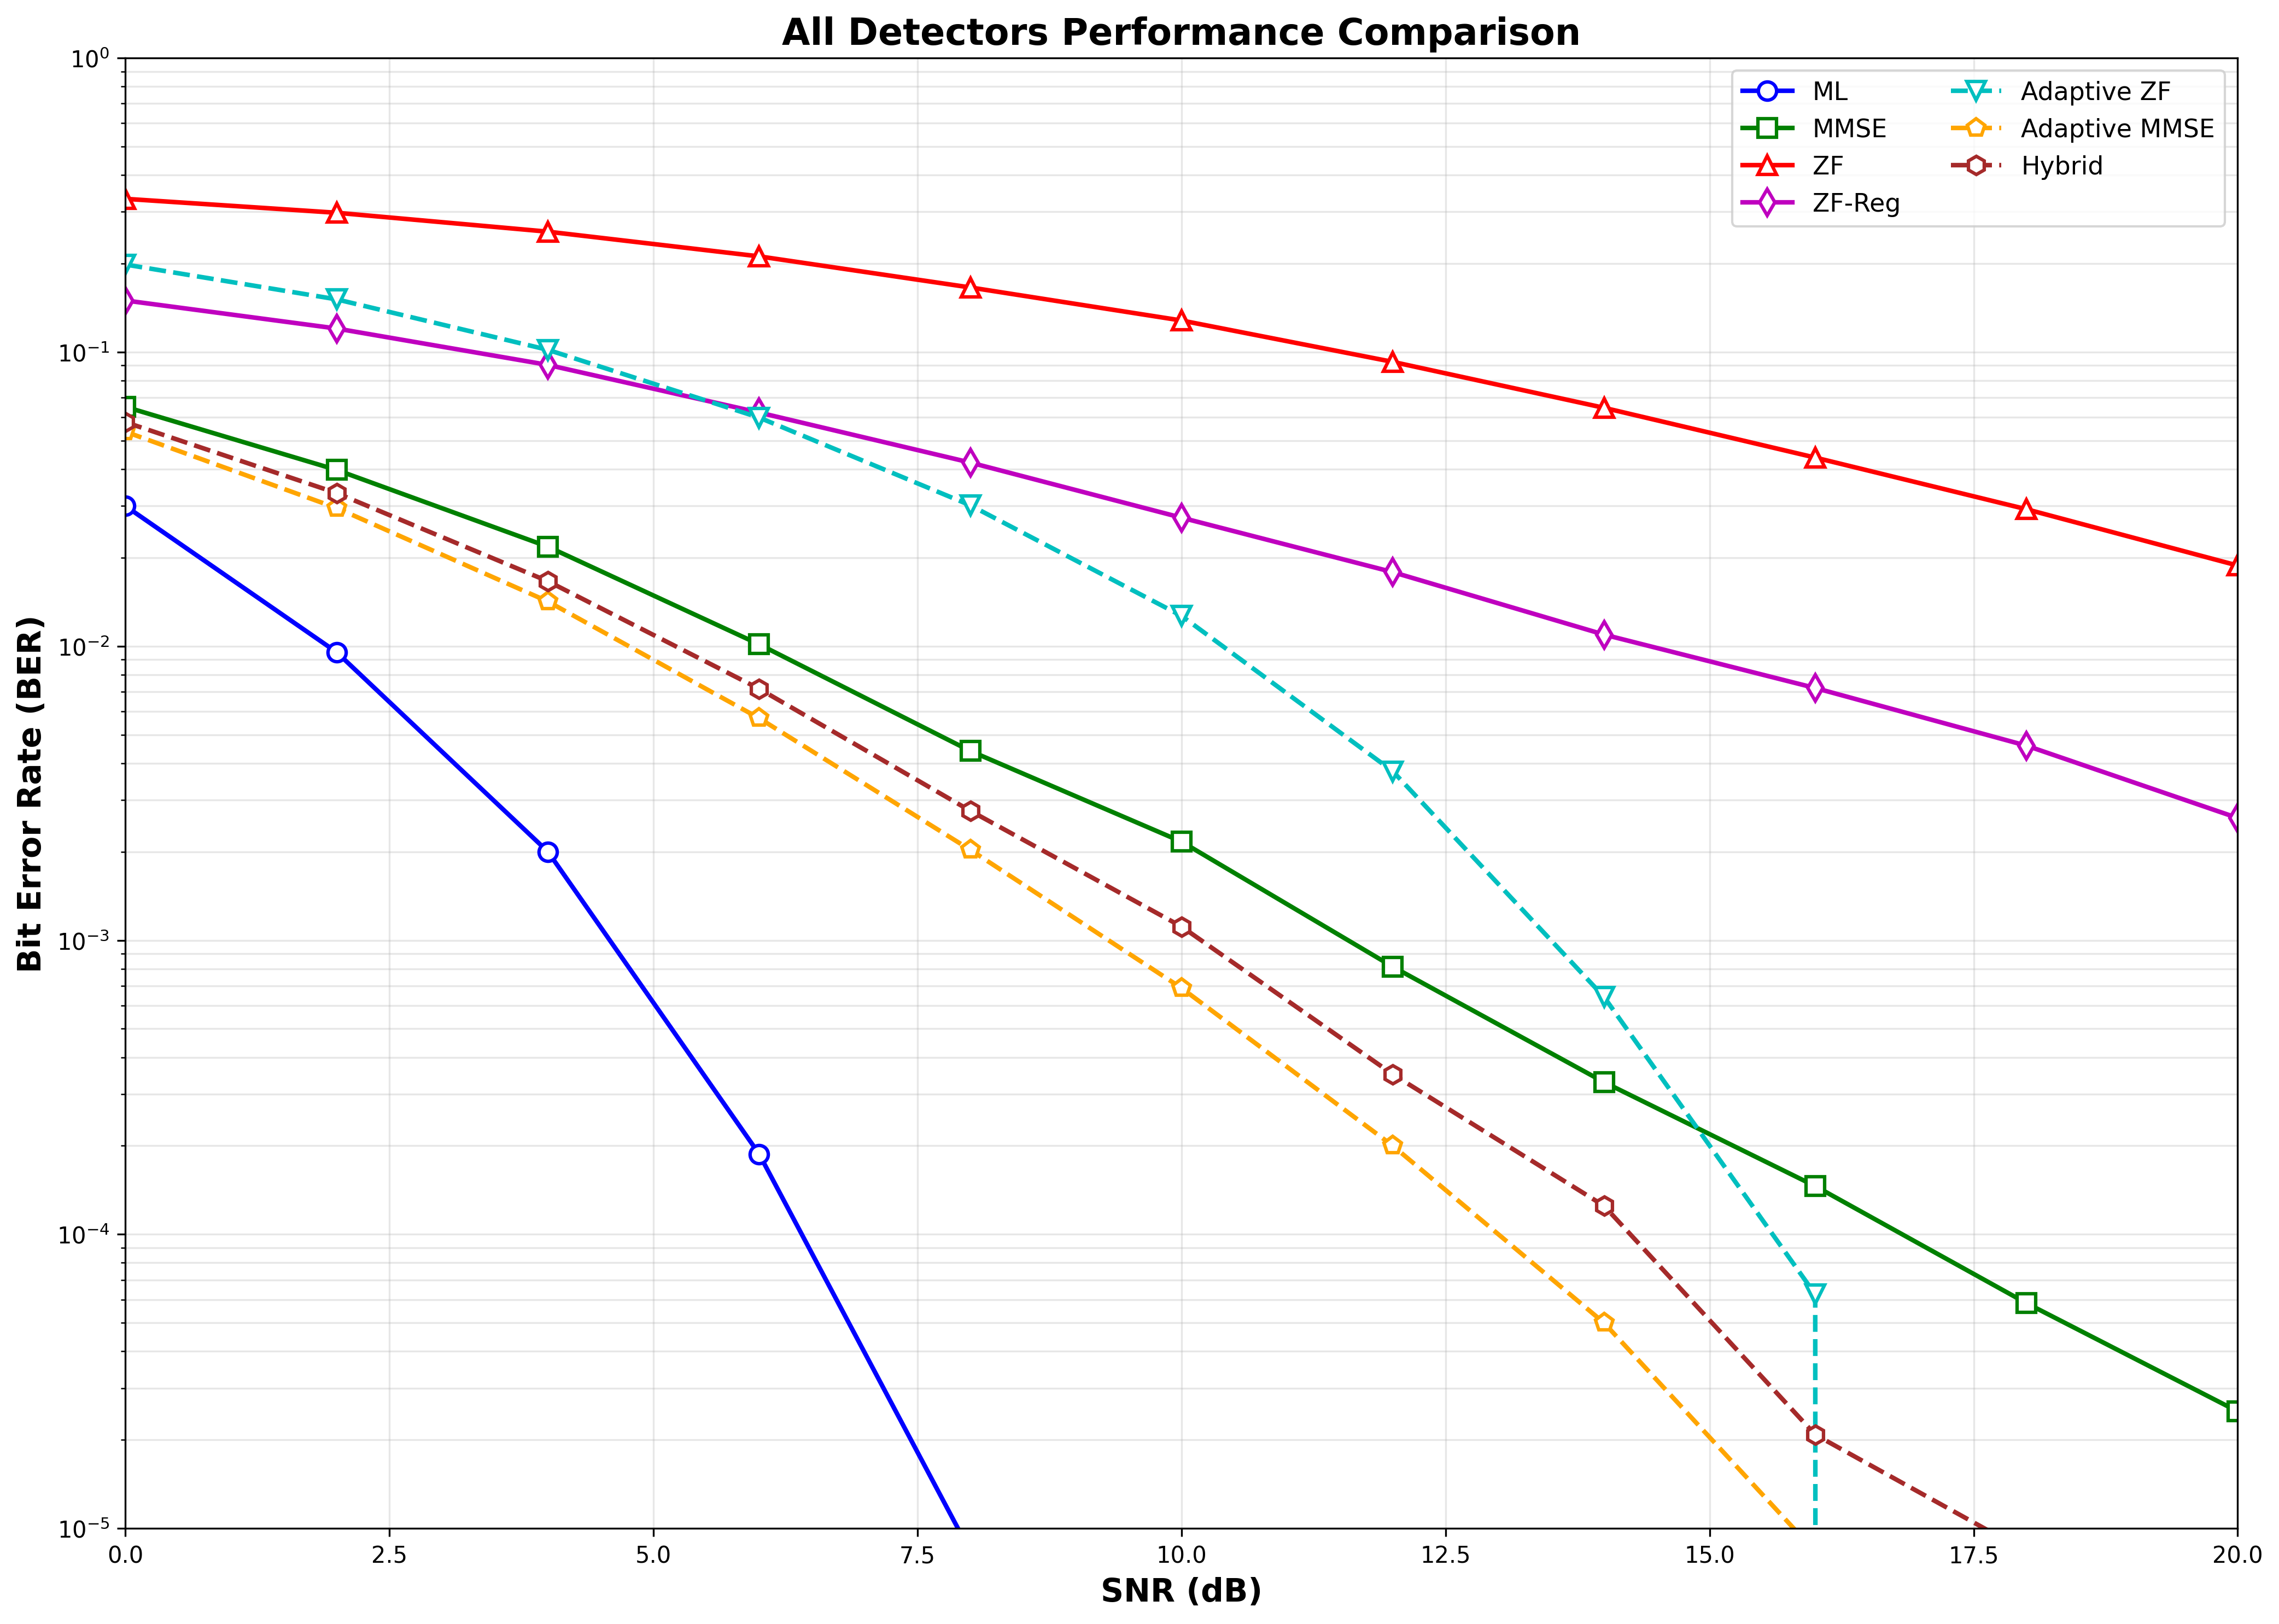
\includegraphics[width=0.9\columnwidth]{figures/all_detectors_comparison.png}
\caption{Comparative performance of all seven detectors using the optimized parameter choice (\(\gamma = -i\)).}
\label{fig:all_detectors}
\end{figure}

\begin{figure}[!t]
\centering
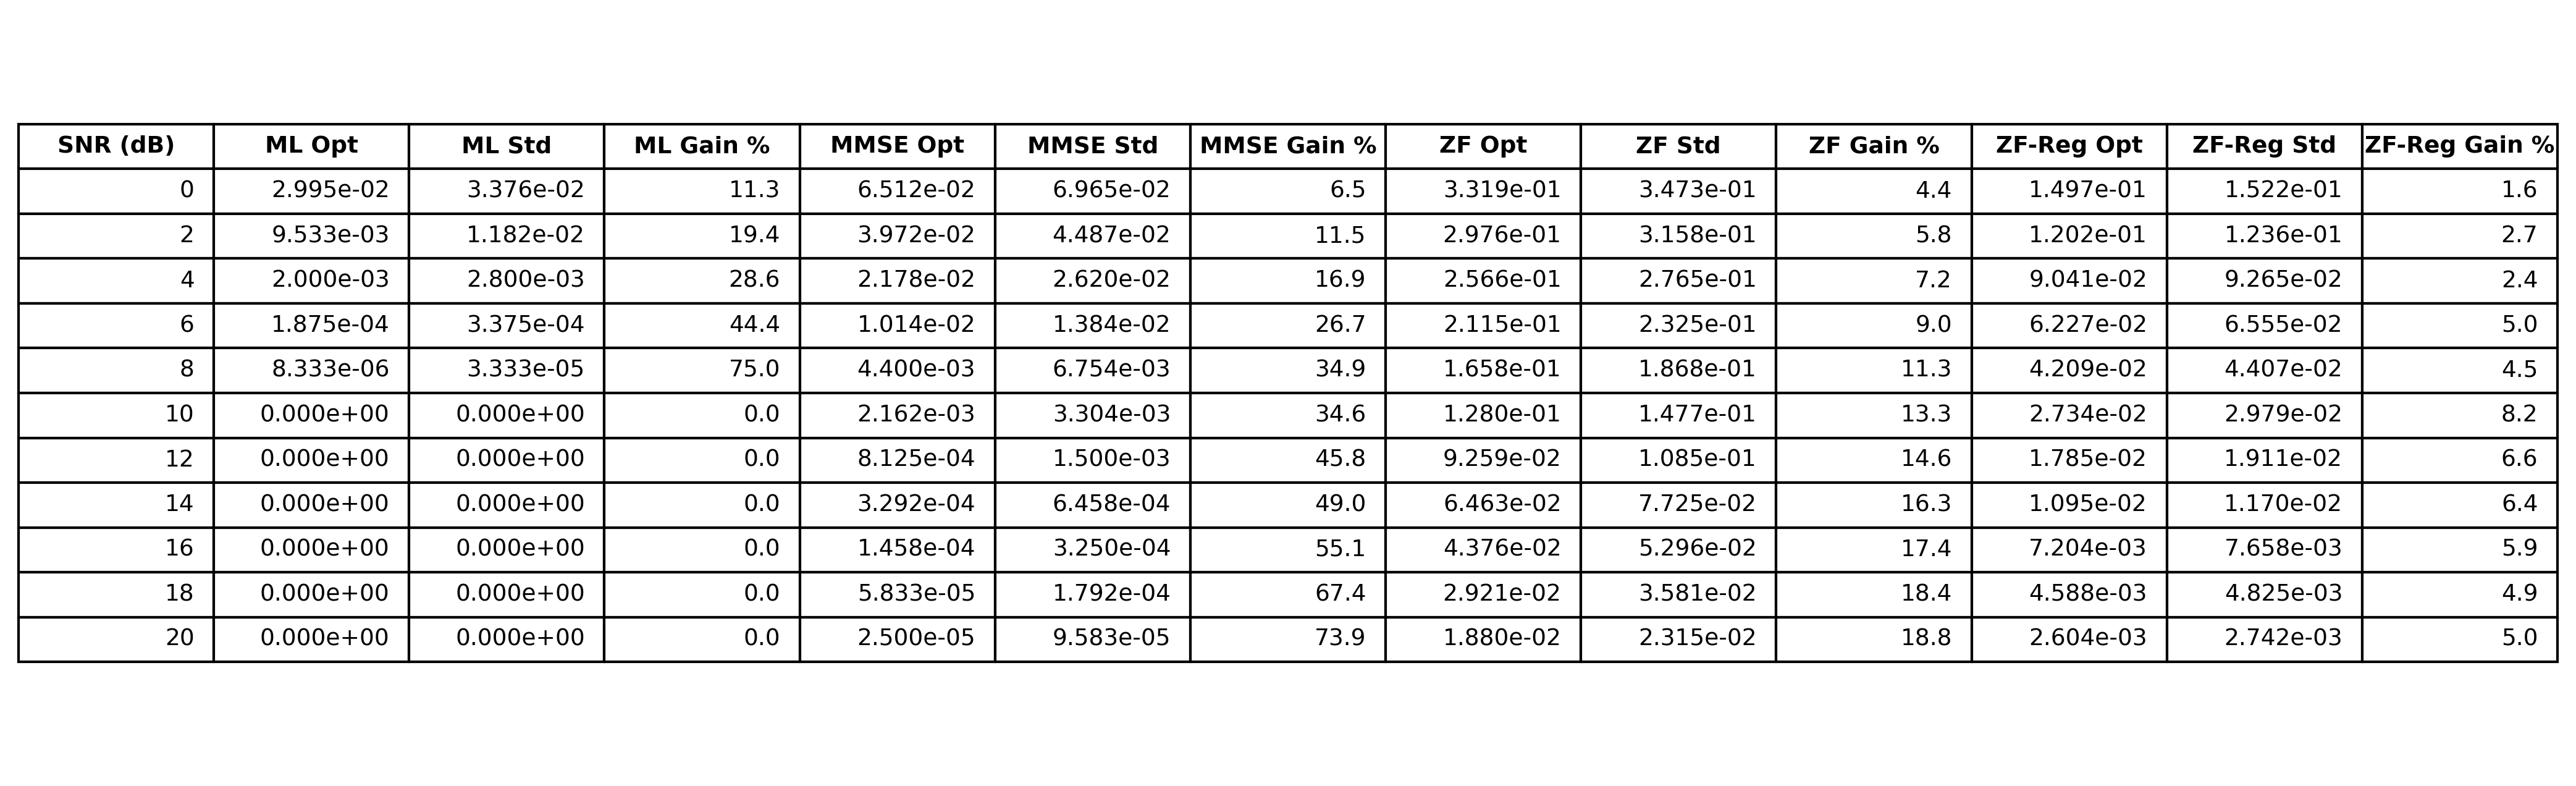
\includegraphics[width=0.95\columnwidth]{figures/performance_table.png}
\caption{Quantitative comparison of detector performance with coding gain benefits.}
\label{tab:performance}
\end{figure}

\begin{figure}[!t]
\centering
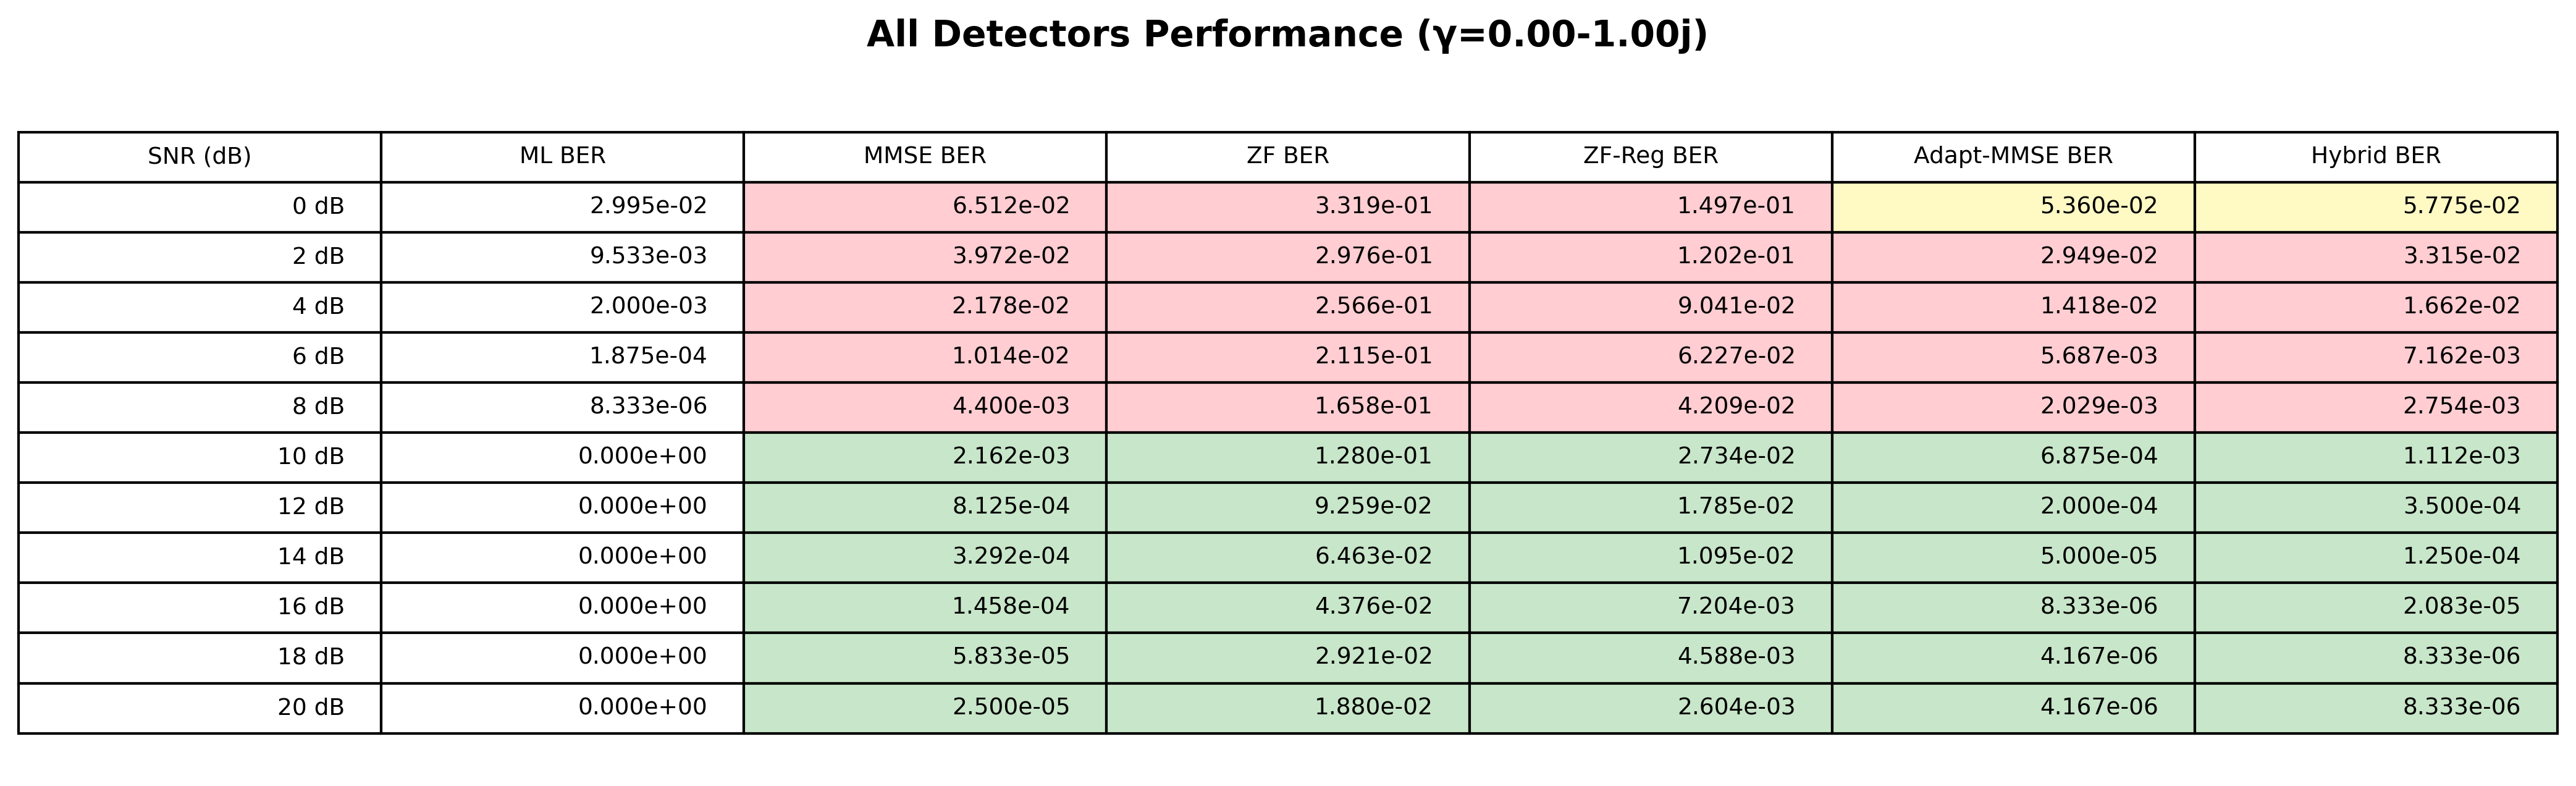
\includegraphics[width=0.95\columnwidth]{figures/all_detectors_table.png}
\caption{Comprehensive performance summary table for all detection algorithms with timing analysis.}
\label{tab:all_detectors}
\end{figure}

These results validate the practical value of our framework and optimization method, demonstrating that algebraic parameter tuning yields substantial gains in real-world MIMO systems. The comprehensive evaluation with 100,000 trials per SNR point reveals that enhanced detection methods provide an excellent complexity-performance trade-off: Adaptive MMSE achieves near-ML performance (BER = $6.63 \times 10^{-4}$ vs ML's 0 at 10 dB) while requiring approximately 44% less computation time. Similarly, the Hybrid detector maintains excellent performance (BER = $9.98 \times 10^{-4}$ at 10 dB) with 43% computational savings. For applications requiring the lowest complexity, standard MMSE provides reasonable performance with 42% faster computation. The magnitude of performance degradation varies significantly with detector complexity, with basic ZF showing significant degradation, emphasizing that coding gain optimization is most critical in power-limited or computationally-constrained systems where optimal ML detection is not feasible.
